%%%%%%%%%%%%%%%%%%%%%%%%%%%%%%%%%%%%%%%%%%%%%%%%%%%%%%%%%%%%%%%%%%%%%%%%%
%  Zawartość: Główny plik szablonu pracy dyplomowej (magisterskiej/inżynierskiej).
%  Opracował: Tomasz Kubik <tomasz.kubik@pwr.edu.pl>
%  Data: kwiecień 2016
%  Wersja: 0.2
%%%%%%%%%%%%%%%%%%%%%%%%%%%%%%%%%%%%%%%%%%%%%%%%%%%%%%%%%%%%%%%%%%%%%%%%%

\documentclass[a4paper,onecolumn,oneside,12pt,extrafontsizes]{memoir}
% W celu przygotowania wydruku do archiwum należy przesłonić komendę powyższą
% dwoma poniższymi komendami:
%\documentclass[a4paper,onecolumn,twoside,10pt]{memoir} 
%\renewcommand{\normalsize}{\fontsize{8pt}{10pt}\selectfont}

%\usepackage[cp1250]{inputenc} % jeśli kodowanie edytowanych plików to cp1250 
\usepackage[utf8]{inputenc} % jeśli kodowanie edytowanych plików to UTF8
\usepackage[T1]{fontenc}
\usepackage[polish]{babel}
%\DisemulatePackage{setspace}
\usepackage{setspace}
\usepackage{tabularx}
\usepackage{color,calc}
%\usepackage{soul} % pakiet z komendami do podkreślania tekstu

\usepackage{ebgaramond} % pakiet z czcionkami garamond, potrzebny tylko do strony tytułowej, musi wystąpić przed pakietem tgtermes

%% Aby uzyskać polskie literki w pdfie (a nie zlepki) korzystamy z pakietu czcionek tgterms. 
%% W pakiecie tym są zdefiniowane klony czcionek Times o kształtach: normalny, pogrubiony, italic, italic pogrubiony.
%% W pakiecie tym brakuje czcionki o kształcie: slanted (podobny do italic). 
%% Jeśli w dokumencie gdzieś zostanie zastosowana czcionka slanted (np. po użyciu komendy \textsl{}), to
%% latex dokona podstawienia na czcionkę standardową i zgłosi to w ostrzeżeniu (warningu).
%% Ponadto tgtermes to czcionka do tekstu. Wszelkie matematyczne wzory będą sformatowane domyślną czcionką do wzorów.
%% Jeśli wzory mają być sformatowane z wykorzystaniem innych czcionek, trzeba to jawnie zadeklarować.

%% Po zainstalowaniu pakietu tgtermes może będzie trzeba zauktualizować informacje 
%% o dostępnych fontach oraz mapy. Można to zrobić z konsoli (jako administrator)
%% initexmf --admin --update-fndb
%% initexmf --admin --mkmaps

\usepackage{tgtermes}   
\renewcommand*\ttdefault{txtt}

% We wcześniejszej wersji szablonu korzystano z innych czcionek. Dla celów historycznych pozostawiono je w komentarzu
%\usepackage{mathptmx} % pakiet będący następcą pakietów times and mathptm, niestety polskie literki są zlepkami
%\usepackage{newtxtext,newtxmath} % pakiety dostarczające Times dla tekstów i wzorów matematycznych,  
%                                  rozwiązuje problemy występujące w mathptmx, ale wymaga zainstalowania
%                                  dodatkowych pakietów oraz uruchomienia updmap (konsola administratora)
%                                  niestety polskie literki są zlepkami
%\usepackage{newtxmath,tgtermes} % można też połączyć czcionki do tekstu i czcionki do wzorów
\usepackage{listings} % pakiet do prezentacji kodu. 
\lstset{
    basicstyle=\ttfamily,
    columns=fullflexible,
    frame=single,
    numbers=left,
    stepnumber=1,
    showstringspaces=false,
    tabsize=1,
    breaklines=true,
    breakatwhitespace=false,
    postbreak=\mbox{\textcolor{red}{$\hookrightarrow$}\space},
}
%Wcześniej był problem z polskimi znakami w otoczeniu lstlisting, stąd pozostawiono w komentarzu zastosowane wtedy rozwiązanie: 
\lstset{literate=%-
{ą}{{\k{a}}}1 {ć}{{\'c}}1 {ę}{{\k{e}}}1 {ł}{{\l{}}}1 {ń}{{\'n}}1 {ó}{{\'o}}1 {ś}{{\'s}}1 {ż}{{\.z}}1 {ź}{{\'z}}1 {Ą}{{\k{A}}}1 {Ć}{{\'C}}1 {Ę}{{\k{E}}}1 {Ł}{{\L{}}}1 {Ń}{{\'N}}1 {Ó}{{\'O}}1 {Ś}{{\'S}}1 {Ż}{{\.Z}}1 {Ź}{{\'Z}}1 }%{\ \ }{{\ }}1}

% Choć możliwe jest zastosowanie różnych pakietów formatujących tabele, zaleca się tego nie robić.
%\usepackage{longtable}
%\usepackage{ltxtable}
%\usepackage{tabulary}

%%%%%%%%%%%%%%%%%%%%%%%%%%%%%%%%%%%%%%%%%%%%%%%%%%%
%% Ustawienia odpowiedzialne za sposób łamania dokumentu
%% i ułożenie elementów pływających
%%%%%%%%%%%%%%%%%%%%%%%%%%%%%%%%%%%%%%%%%%%%%%%%%%%
%\hyphenpenalty=10000		% nie dziel wyrazów zbyt często
\clubpenalty=10000      %kara za sierotki
\widowpenalty=10000  % nie pozostawiaj wdów
\brokenpenalty=10000		% nie dziel wyrazów między stronami
\exhyphenpenalty=999999		% nie dziel słów z myślnikiem
\righthyphenmin=3			% dziel minimum 3 litery

%\tolerance=4500
%\pretolerance=250
%\hfuzz=1.5pt
%\hbadness=1450

\renewcommand{\topfraction}{0.95}
\renewcommand{\bottomfraction}{0.95}
\renewcommand{\textfraction}{0.05}
\renewcommand{\floatpagefraction}{0.35}

%%%%%%%%%%%%%%%%%%%%%%%%%%%%%%%%%%%%%%%%%%%%%%%%%%%
%%  Ustawienia rozmiarów: tekstu, nagłówka i stopki, marginesów
%%  dla dokumentów klasy memoir 
%%%%%%%%%%%%%%%%%%%%%%%%%%%%%%%%%%%%%%%%%%%%%%%%%%%
\setlength{\headsep}{10pt} 
\setlength{\headheight}{13.6pt} % wartość baselineskip dla czcionki 11pt tj. \small wynosi 13.6pt
\setlength{\footskip}{\headsep+\headheight}
\setlength{\uppermargin}{\headheight+\headsep+1cm}
\setlength{\textheight}{\paperheight-\uppermargin-\footskip-1.5cm}
\setlength{\textwidth}{\paperwidth-5cm}
\setlength{\spinemargin}{2.5cm}
\setlength{\foremargin}{2.5cm}
\setlength{\marginparsep}{2mm}
\setlength{\marginparwidth}{2.3mm}
%\settrimmedsize{297mm}{210mm}{*}
%\settrims{0mm}{0mm}	
\checkandfixthelayout[fixed] % konieczne, aby się dobrze wszystko poustawiało
%%%%%%%%%%%%%%%%%%%%%%%%%%%%%%%%%%%%%%%%%%%%%%%%
%%  Ustawienia odległości linii, wcięć, odstępów
%%%%%%%%%%%%%%%%%%%%%%%%%%%%%%%%%%%%%%%%%%%%%%%%
\linespread{1}
%\linespread{1.241}
\setlength{\parindent}{14.5pt}
%\setbeforesecskip{10pt plus 0.5ex}%{-3.5ex \@plus -1ex \@minus -.2ex}
%\setaftersecskip{10pt plus 0.5ex}%\onelineskip}
%\setbeforesubsecskip{8pt plus 0.5ex}%{-3.5ex \@plus -1ex \@minus -.2ex}
%\setaftersubsecskip{8pt plus 0.5ex}%\onelineskip}
%\setlength\floatsep{6pt plus 2pt minus 2pt} 
%\setlength\intextsep{12pt plus 2pt minus 2pt} 
%\setlength\textfloatsep{12pt plus 2pt minus 2pt} 

%%%%%%%%%%%%%%%%%%%%%%%%%%%%%%%%%%%%%%%%%%%%%%%%%%%
%%  Pakiety i komendy zastosowane tylko do zamieszczenia informacji o użytych komendach i fontach
%%  Normalnie nie są potrzebne, można je zamarkować podczas redakcji pracy
%%%%%%%%%%%%%%%%%%%%%%%%%%%%%%%%%%%%%%%%%%%%%%%%%%%
\usepackage{memlays}     % extra layout diagrams, zastosowane w szblonie do 'debuggowania', używa pakietu layouts
%\usepackage{layouts}
\usepackage{printlen} % pakiet do wyświetlania wartości zdefiniowanych długości, stosowany do 'debuggowania'
\uselengthunit{pt}
\makeatletter
\newcommand{\showFontSize}{\f@size pt} % makro wypisujące wielkość bieżącej czcionki
\makeatother
% do pokazania ramek można byłoby użyć:
%\usepackage{showframe} 


%%%%%%%%%%%%%%%%%%%%%%%%%%%%%%%%%%%%%%%%%%%%%%%%%%%
%%  Formatowanie list wyliczeniowych, wypunktowań i własnych otoczeń
%%%%%%%%%%%%%%%%%%%%%%%%%%%%%%%%%%%%%%%%%%%%%%%%%%%

% Domyślnie wypunktowania mają zadeklatorowane znaki, które nie występują w tgtermes
% Aby latex nie podstawiał w ich miejsca znaków z czcionki standardowej można zrobić podstawienie:
%    \DeclareTextCommandDefault{\textbullet}{\ensuremath{\bullet}}
%    \DeclareTextCommandDefault{\textasteriskcentered}{\ensuremath{\ast}}
%    \DeclareTextCommandDefault{\textperiodcentered}{\ensuremath{\cdot}}
% Jednak jeszcze lepszym pomysłem jest zdefiniowanie otoczeń z wykorzystaniem enumitem
\usepackage{enumitem} % pakiet pozwalający zarządzać formatowaniem list wyliczeniowych
\setlist{noitemsep,topsep=4pt,parsep=0pt,partopsep=4pt,leftmargin=*} % zadeklarowane parametry pozwalają uzyskać 'zwartą' postać wypunktowania bądź wyliczenia
\setenumerate{labelindent=0pt,itemindent=0pt,leftmargin=!,label=\arabic*.} % można zmienić \arabic na \alph, jeśli wyliczenia mają być z literkami
\setlistdepth{4} % definiujemy głębokość zagnieżdżenia list wyliczeniowych do 4 poziomów
\setlist[itemize,1]{label=$\bullet$}  % definiujemy, jaki symbol ma być użyty w wyliczeniu na danym poziomie
\setlist[itemize,2]{label=\normalfont\bfseries\textendash}
\setlist[itemize,3]{label=$\ast$}
\setlist[itemize,4]{label=$\cdot$}
\renewlist{itemize}{itemize}{4}

%%%http://tex.stackexchange.com/questions/29322/how-to-make-enumerate-items-align-at-left-margin
%\renewenvironment{enumerate}
%{
%\begin{list}{\arabic{enumi}.}
%{
%\usecounter{enumi}
%%\setlength{\itemindent}{0pt}
%%\setlength{\leftmargin}{1.8em}%{2zw} % 
%%\setlength{\rightmargin}{0zw} %
%%\setlength{\labelsep}{1zw} %
%%\setlength{\labelwidth}{3zw} % 
%\setlength{\topsep}{6pt}%
%\setlength{\partopsep}{0pt}%
%\setlength{\parskip}{0pt}%
%\setlength{\parsep}{0em} % 
%\setlength{\itemsep}{0em} % 
%%\setlength{\listparindent}{1zw} % 
%}
%}{
%\end{list}
%}

\makeatletter
\renewenvironment{quote}{
	\begin{list}{}
	{
	\setlength{\leftmargin}{1em}
	\setlength{\topsep}{0pt}%
	\setlength{\partopsep}{0pt}%
	\setlength{\parskip}{0pt}%
	\setlength{\parsep}{0pt}%
	\setlength{\itemsep}{0pt}
	}
	}{
	\end{list}}
\makeatother

%%%%%%%%%%%%%%%%%%%%%%%%%%%%%%%%%%%%%%%%%
%%  Pakiet do generowania indeksu (ważne, aby wstawić przed hyperref)
%%%%%%%%%%%%%%%%%%%%%%%%%%%%%%%%%%%%%%%%%
\DisemulatePackage{imakeidx}
\usepackage[makeindex,noautomatic]{imakeidx} % tutaj mówimy, żeby indeks nie generował się automatycznie, 

%\usepackage[noautomatic]{imakeidx} 
\makeindex

\makeatletter
%%%\renewenvironment{theindex}
							 %%%{\vskip 10pt\@makeschapterhead{\indexname}\vskip -3pt%
								%%%\@mkboth{\MakeUppercase\indexname}%
												%%%{\MakeUppercase\indexname}%
								%%%\vspace{-3.2mm}\parindent\z@%
								%%%\renewcommand\subitem{\par\hangindent 16\p@ \hspace*{0\p@}}%%
								%%%\phantomsection%
								%%%\begin{multicols}{2}
								%%%%\thispagestyle{plain}
								%%%\parindent\z@                
								%%%%\parskip\z@ \@plus .3\p@\relax
								%%%\let\item\@idxitem}
							 %%%{\end{multicols}\clearpage}
%%%
\makeatother


\usepackage{ifpdf}
%\newif\ifpdf \ifx\pdfoutput\undefined
%\pdffalse % we are not running PDFLaTeX
%\else
%\pdfoutput=1 % we are running PDFLaTeX
%\pdftrue \fi
\ifpdf
 \usepackage[pdftex,bookmarks,breaklinks,unicode]{hyperref}
 \usepackage[pdftex]{graphicx}
 \DeclareGraphicsExtensions{.pdf,.jpg,.mps,.png}
\pdfcompresslevel=9
\pdfoutput=1
\makeatletter
\AtBeginDocument{
  \hypersetup{
	pdfinfo={
    Title = {\@title},
    Author = {\@author},
    Subject={},
    Keywords={słowa kluczowe},
  }}
}
\makeatother
\else
\usepackage{graphicx}
\DeclareGraphicsExtensions{.eps,.ps,.jpg,.mps,.png}
\fi
\sloppy


%\graphicspath{{rys01/}{rys02/}}


%%%%%%%%%%%%%%%%%%%%%%%%%%%%%%%%%%%%%%%%%
% Metadane dla pdfa


%\ifpdf
%\pdfinfo{
   %/Author (Nicola Talbot)
   %/Title  (Creating a PDF document using PDFLaTeX)
   %/CreationDate (D:20040502195600)
   %/ModDate (D:\pdfdate)
   %/Subject (PDFLaTeX)
   %/Keywords (PDF;LaTeX)
%}
%\fi

% Deklaracja głębokościu numeracji
\setcounter{secnumdepth}{2}
\setcounter{tocdepth}{2}
\setsecnumdepth{subsection} % activating subsubsec numbering in doc


% Kropki po numerach sekcji
\makeatletter
\def\@seccntformat#1{\csname the#1\endcsname.\quad}
\def\numberline#1{\hb@xt@\@tempdima{#1\if&#1&\else.\fi\hfil}}
\makeatother

\renewcommand{\chapternumberline}[1]{#1.\quad}
\renewcommand{\cftchapterdotsep}{\cftdotsep}

%\definecolor{niceblue}{rgb}{.168,.234,.671}

% Czcionka do podpisów tabel i rysunków
\captionnamefont{\small}
\captiontitlefont{\small}
% makro pozwalające zmienić sposób wypisywania rozdziału
%\def\printchaptertitle##1{\fonttitle \space \thechapter.\space ##1} 

%\usepackage{ltcaption}
% The ltcaption package supports \CaptionLabelFont & \CaptionTextFont introduced by the NTG document classes
%\renewcommand\CaptionLabelFont{\small}
%\renewcommand\CaptionTextFont{\small}

% Przedefiniowanie etykiet w podpisach tabel i rysunków
%\AtBeginDocument{% 
        \addto\captionspolish{% 
        \renewcommand{\tablename}{Tab.}% 
}%} 

%\AtBeginDocument{% 
%        \addto\captionspolish{% 
%        \renewcommand{\chaptername}{Rozdział}% 
%}} 

%\AtBeginDocument{% 
        \addto\captionspolish{% 
        \renewcommand{\figurename}{Rys.}% 
}%}


%\AtBeginDocument{% 
        \addto\captionspolish{% 
        \renewcommand{\bibname}{Literatura}% 
}%}

%\AtBeginDocument{% 
        \addto\captionspolish{% 
        \renewcommand{\listfigurename}{Spis rysunków}% 
}%}

%\AtBeginDocument{% 
        \addto\captionspolish{% 
        \renewcommand{\listtablename}{Spis tabel}% 
}%}

%\AtBeginDocument{% 
        \addto\captionspolish

%%%%%%%%%%%%%%%%%%%%%%%%%%%%%%%%%%%%%%%%%%%%%%%%%%%%%%%%%%%%%%%%%%                  
%% Definicje stopek i nagłówków
%%%%%%%%%%%%%%%%%%%%%%%%%%%%%%%%%%%%%%%%%%%%%%%%%%%%%%%%%%%%%%%%%%                  
\addtopsmarks{headings}{%
\nouppercaseheads % added at the beginning
}{%
\createmark{chapter}{both}{shownumber}{}{. \space}
%\createmark{chapter}{left}{shownumber}{}{. \space}
\createmark{section}{right}{shownumber}{}{. \space}
}%use the new settings

\makeatletter
\copypagestyle{outer}{headings}
\makeoddhead{outer}{}{}{\small\itshape\rightmark}
\makeevenhead{outer}{\small\itshape\leftmark}{}{}
\makeoddfoot{outer}{\small\@author:~\@titleShort}{}{\small\thepage}
\makeevenfoot{outer}{\small\thepage}{}{\small\@author:~\@title}
\makeheadrule{outer}{\linewidth}{\normalrulethickness}
\makefootrule{outer}{\linewidth}{\normalrulethickness}{2pt}
\makeatother

% fix plain
\copypagestyle{plain}{headings} % overwrite plain with outer
\makeoddhead{plain}{}{}{} % remove right header
\makeevenhead{plain}{}{}{} % remove left header
\makeevenfoot{plain}{}{}{}
\makeoddfoot{plain}{}{}{}

\copypagestyle{empty}{headings} % overwrite plain with outer
\makeoddhead{empty}{}{}{} % remove right header
\makeevenhead{empty}{}{}{} % remove left header
\makeevenfoot{empty}{}{}{}
\makeoddfoot{empty}{}{}{}


%%%%%%%%%%%%%%%%%%%%%%%%%%%%%%%%%%%%%%%
%% Definicja strony tytułowej 
%%%%%%%%%%%%%%%%%%%%%%%%%%%%%%%%%%%%%%%
\makeatletter
%Uczelnia
\newcommand\uczelnia[1]{\renewcommand\@uczelnia{#1}}
\newcommand\@uczelnia{}
%Wydział
\newcommand\wydzial[1]{\renewcommand\@wydzial{#1}}
\newcommand\@wydzial{}
%Kierunek
\newcommand\kierunek[1]{\renewcommand\@kierunek{#1}}
\newcommand\@kierunek{}
%Specjalność
\newcommand\specjalnosc[1]{\renewcommand\@specjalnosc{#1}}
\newcommand\@specjalnosc{}
%Tytuł po angielsku
\newcommand\titleEN[1]{\renewcommand\@titleEN{#1}}
\newcommand\@titleEN{}
%Tytuł krótki
\newcommand\titleShort[1]{\renewcommand\@titleShort{#1}}
\newcommand\@titleShort{}
%Promotor
\newcommand\promotor[1]{\renewcommand\@promotor{#1}}
\newcommand\@promotor{}

%\usepackage[absolute]{textpos} % zamarkowano, bo ostatecznie wykorzystano otoczenie picture

\def\maketitle{%
  \pagestyle{empty}%
%%\garamond 
	\fontfamily{\ebgaramond@family}\selectfont % na stronie tytułowej czcionka garamond
%%%%%%%%%%%%%%%%%%%%%%%%%%%%%%%%%%%%%	
%% Poniżej, w otoczniu picture, wstawiono tytuł i autora. 
%% Tytuł (z autorem) musi znaleźć się w obszarze 
%% odpowiadającym okienku 110mmx75mm, którego lewy górny róg 
%% jest w położeniu 77mm od lewej i 111mm od górnej  krawędzi strony 
%% (tak wynika z wycięcia na okładce). 
%% Poniższy kod musi być użyty dokładnie w miejscu gdzie jest.
%% Jeśli tytuł nie mieści się w okienku, to należy tak pozmieniać 
%% parametry użytych komend, aby ten przydługi tytuł jednak 
%% upakować go do okienka.
%%
%% Sama okładka (kolorowa strona z wycięciem, do pobrania z dydaktyki) 
%% powinna być przycięta o 3mm od każdej z krawędzi.
%% Te 3mm pewnie zostawiono na ewentualne spady czy też specjalną oprawę.
%%%%%%%%%%%%%%%%%%%%%%%%%%%%%%%%%%%%%	
\newlength{\tmpfboxrule}
\setlength{\tmpfboxrule}{\fboxrule}
\setlength{\fboxsep}{2mm}
\setlength{\fboxrule}{0mm} 
%\setlength{\fboxrule}{0.1mm} %% jeśli chcemy zobaczyć ramkę
\setlength{\unitlength}{1mm}
\begin{picture}(0,0)
\put(26,-124){\fbox{
\parbox[c][71mm][c]{104mm}{\centering%\lineskip=34pt 
\fontsize{16pt}{18pt}\selectfont \@title\\[5mm]
\fontsize{16pt}{18pt}\selectfont \@titleEN\\[20mm]
\fontsize{16pt}{18pt}\selectfont AUTOR:\\[2mm]
\fontsize{14pt}{16pt}\selectfont \@author}
}
}
\end{picture}
\setlength{\fboxrule}{\tmpfboxrule} 
%%%%%%%%%%%%%%%%%%%%%%%%%%%%%%%%%%%%%
%% Reszta strony z nazwą uczelni, wydziału, kierunkiem, specjalnością
%% promotorem, oceną pracy, miastem i rokiem
	{\centering%\vspace{-1cm}
		{\fontsize{22pt}{24pt}\selectfont \@uczelnia}\\[0.4cm]
		{\fontsize{22pt}{24pt}\selectfont \@wydzial}\\[0.5cm]
		  \hrule %\vspace*{0.7cm}
	}
{\flushleft\fontsize{14pt}{16pt}\selectfont%
\begin{tabular}{ll}
KIERUNEK: & \@kierunek\\
SPECJALNOŚĆ: & \@specjalnosc\\
\end{tabular}\\[1.3cm]
}
{\centering
{\fontsize{32pt}{36pt}\selectfont PRACA DYPLOMOWA}\\[0.5cm]
{\fontsize{32pt}{36pt}\selectfont INŻYNIERSKA}\\[2.5cm]
}
\vfill
\begin{tabularx}{\linewidth}{p{6cm}l}
		&{\fontsize{16pt}{18pt}\selectfont PROWADZĄCY PRACĘ:}\\[2mm] %UWAGA: tutaj jest miejsce na nazwisko promotora pracy
		&{\fontsize{14pt}{16pt}\selectfont \@promotor}\\[10mm]
		&{\fontsize{16pt}{18pt}\selectfont OCENA PRACY:}\\[20mm]
	\end{tabularx}
\vspace{2cm}
\hrule\vspace*{0.3cm}
{\centering
{\fontsize{16pt}{18pt}\selectfont \@date}\\[0cm]
}
%\ungaramond
\normalfont
 \cleardoublepage
}
\makeatother
%%%%%%%%%%%%%%%%%%%%%%%%%%%%%%%%%%%%%%%%%

%\AtBeginDocument{\addtocontents{toc}{\protect\thispagestyle{empty}}}




%%%%%%%%%%%%%%%%%%%%%%%%%%%%%%%%%%%%%%%%%
%%  Metadane dokumentu 
%%%%%%%%%%%%%%%%%%%%%%%%%%%%%%%%%%%%%%%%%
\title{Projekt oraz implementacja aplikacji w C\# do ewidencji księgowej danych kontrahentów i fakturowania}
\titleShort{Projekt oraz implementacja aplikacji w C\#... }
\titleEN{Project and application implementation in C\# to the accounting records of contractors' data and invoicing}
\author{Mateusz Polok}
\uczelnia{POLITECHNIKA WROCŁAWSKA}
\wydzial{WYDZIAŁ ELEKTRONIKI}
\kierunek{INFORMATYKA}
\specjalnosc{SYSTEMY I SIECI KOMPUTEROWE}
\promotor{Dr inż. Mariusz Topolski, W-4/K-2}
\date{WROCŁAW, 2019}

% Ustawienie odstępu od góry w nienumerowanych rozdziałach oraz wykazach:
% Spis treści, Spis tabel, Spis rysunków, Indeks rzeczowy

%\newlength{\linespace}
%\setlength{\linespace}{-\beforechapskip-\topskip+\headheight+\topsep}
%\makechapterstyle{noNumbered}{%
%\renewcommand\chapterheadstart{\vspace*{\linespace}}
%}

%% powyższa komenda załatwia to, co robią komendy poniższe dla spisów
%\renewcommand*{\tocheadstart}{\vspace*{\linespace}}
%\renewcommand*{\lotheadstart}{\vspace*{\linespace}}
%\renewcommand*{\lofheadstart}{\vspace*{\linespace}}

%%%%%%%%%%%%%%%%%%%%%%%%%%%%%%%%%%%%%%%%%
%                  Początek dokumentu 
%%%%%%%%%%%%%%%%%%%%%%%%%%%%%%%%%%%%%%%%%
%\includeonly{skroty,rozdzial01} % jeśli chcemy kompilować tylko fragmenty, to można tu je wpisać

\begin{document}
% Tutaj można przełączyć odstęp między liniami
%\SingleSpacing
%\OnehalfSpacing
%\DoubleSpacing

%\settypeoutlayoutunit{cm} % do debugowania
%\typeoutstandardlayout    % wypisuje na stdout informacje o ustawieniach
\maketitle

\newpage

\chapterstyle{noNumbered}
\pagestyle{outer}
\mbox{}\pdfbookmark[0]{Spis treści}{spisTresci.1}
\tableofcontents* 

\newpage
\mbox{}\pdfbookmark[0]{Spis rysunków}{spisRysunkow.1}
%\addcontentsline{toc}{chapter}{Spis rysunków}
\listoffigures*
\begin{flushleft}

\end{flushleft}
%{%
%\let\oldnumberline\numberline%
%\renewcommand{\numberline}{\figurename~\oldnumberline}%
%\listoffigures%
%}


\newpage
\mbox{}\pdfbookmark[0]{Spis tabel}{spisTabel.1}
%\addcontentsline{toc}{chapter}{Spis tabel}
\listoftables*

\chapter*{Skróty}\mbox{}\pdfbookmark[0]{Skróty}{skroty.1}
\label{sec:skroty}
\noindent
\begin{description}
  \item [CRUD] (ang.\ \emph{Create, Read, Update, Delete })
  \item [EF Core] (ang.\ \emph{Entity Framework Core})
  \item [DI] (ang.\ \emph{Dependency Injection})
  \item [WPF] (ang.\ \emph{Windows Presentation Foundation}

\end{description}
 %skróty można sobie pominąć
\chapterstyle{default}
\chapter{Wstęp}
\section{Cel i zakres pracy}
Celem pracy jest zrobienie projektu oraz jego zaimplementowanie w formie aplikacji do ewidencji księgowej danych kontrahentów i fakturowania. Należy opracować algorytmy wspomagające prowadzenie faktur oraz zarządanie danymi kontrahentów. W zakres pracy wchodzi:
\begin{itemize}
    \item poznanie silnika graficznego do stworzenia aplikacji desktopowej
    \item wykonanie projektu aplikacji komputerowej
    \item opracowanie bazy danych
    \item implementacja aplikacji
\end{itemize}
W projekcie zostanie użyty język C\# oraz silnik graficzny Windows Presentation Foundation (WPF).

\section{Układ pracy}


\chapter{Analiza wymagań użytkownika}

Aplikacja skierowana jest do każdego użytkownika lub firmy, który potrzebuje systemy, w którym będzie mógł wprowadzać faktury VAT lub pro forma. Ponadto oprogramowanie umożliwa także generowanie PDFów z wybranych przez użytkownika faktur. Interfejs aplikacji jest bardzo intuicyjny oraz prosty w obsłudze, także każda osoba, będzie potrafiła z niego korzystać.

\section{Wymagania funkcjonalne}
\begin{enumerate}
    \item Użytkownik ma możliwość dodania kontrahenta/sprzedawcę \\
    \textbf{Opis: } Każdy użytkownik po wejściu w odpowiednią zakładkę ma możliwość dodania nowego klienta. Klient może zostać dodany również z widoku dodawania faktury.\\
    \textbf{Przebieg: }
    \begin{enumerate}
        \item Użytkownik uzupełnia wymagane pola (nazwa firmy, miasto, ulica, numer domu) oraz może uzupełnić pola opcjonalne (kod pocztowy, numer lokalu, numer telefonu, NIP, REGON, numer konta bankowego, uwagi).
        \item Aplikacja sprawdza poprawność wpisanych danych (w przypadku błędnie podanych, wyświetla stosowny komunikat).
        \item Kontrahent/Sprzedawca zostaje dodany do bazy danych oraz wyświetla się na liście dostępnych już klientów.\\
    \end{enumerate}
    
    \item Użytkownik ma możliwość usunięcia kontrahenta/sprzedawcy\\
    \textbf{Opis: } Każdy użytkownik ma możliwość wybrania dowolnego sprzedawcy/kontrahenta i usunięcia go.\\
    \textbf{Przebieg: } 
    \begin{enumerate}
        \item Użytkownik wybiera sprzedawcę/kontrahenta z listy dostępnych.
        \item Użytkownik klika w odpowiedni przycisk i potwierdza usunięcie.\\
    \end{enumerate}
    
    \item Użytkownik ma możliwość edytowania kontrahenta/sprzedawcy\\
    \textbf{Opis: } Każdy użytkownik po wybraniu konkretnego kontrahenta/sprzedawcy ma możliwość edytowania go.\\
    \textbf{Przebieg: }
    \begin{enumerate}
        \item Po wybraniu konkretnego sprzedawcy/kontrahenta użytkownikowi ukazuje się menu podglądu.
        \item Po przejściu do trybu edycji użytkownik może edytować wszystkie pola.
        \item Użytkownik zatwierdza wprowadzone zmiany.
        \item Wprowadzone zmiany zostają zaktualizowane na liście.\\
    \end{enumerate}
    
    \item Użytkownik ma możliwość dodania faktury \\
    \textbf{Opis: } Każdy użytkownik po wejściu w odpowiednią zakładkę ma możliwość dodania nowej faktury.\\
    \textbf{Przebieg: }
    \begin{enumerate}
        \item Użytkownik uzupełnia wymagane pola (kontrahent, sprzedawca, data wystawienia faktury, termin płatności) oraz może uzupełnić pola opcjonalne (kiedy faktura została opłacona, dodanie nowych pozycji do faktury, uwagi).
        \item Numer faktury jest kolejnym numerem porządkowym ostatniej faktury (np. ostatnia faktura 1/2019, następna faktura 2/2019), przy rozpoczęciu nowego roku, numeracja faktur rozpoczyna się od początku.
        \item Aplikacja sprawdza poprawność wpisanych danych (w przypadku błędnie podanych, wyświetla stosowny komunikat).
        \item Faktura zostaje dodana do bazy danych oraz wyświetla się na liście dostępnych już faktur.\\
    \end{enumerate}
    
    \item Użytkownik ma możliwość usunięcia faktury\\
    \textbf{Opis: } Każdy użytkownik ma możliwość wybrania dowolnej faktury i usunięcia jej.\\
    \textbf{Przebieg: } 
    \begin{enumerate}
        \item Użytkownik wybiera fakturę z listy dostępnych.
        \item Użytkownik klika w odpowiedni przycisk i potwierdza usunięcie.
        \item W przypadku, gdy użytkownik usuwa ostatnią fakturę z danego roku, numeracja faktur się cofa (np. mamy faktury 1/2019, 2/2019, 3/2019, użytkownik usuwa fakturę 3/2019, czyli następna nowa faktura będzie miała numer usuniętej faktury 3/2019).\\
    \end{enumerate}
    
    \item Użytkownik ma możliwość edytowania faktury\\
    \textbf{Opis: } Każdy użytkownik po wybraniu konkretnej faktury ma możliwość edytowania jej.\\
    \textbf{Przebieg: }
    \begin{enumerate}
        \item Po wybraniu konkretnej faktury, użytkownikowi ukazuje się menu podglądu.
        \item Po przejściu do trybu edycji użytkownik może edytować wszystkie pola.
        \item Użytkownik zatwierdza wprowadzone zmiany.
        \item Wprowadzone zmiany zostają zaktualizowane na liście.\\
    \end{enumerate}
    
        \item Użytkownik ma możliwość dodania pozycji na fakturze \\
    \textbf{Opis: } Każdy użytkownik po utworzeniu nowej faktury, ma możliwość dodania nowej pozycji do faktury.\\
    \textbf{Przebieg: }
    \begin{enumerate}
        \item Użytkownik uzupełnia wymagane pola (nazwa produktu, ilość, VAT [\%], jednostka, cena netto lub brutto) i opcjonalne pola PKWiU oraz uwagi.
        \item Aplikacja sprawdza poprawność wpisanych danych (w przypadku błędnie podanych, wyświetla stosowny komunikat).
        \item Pozycja zostaje dodana do faktury oraz wyświetla się na liście pozycji.
    \end{enumerate}
    
    \item Użytkownik ma możliwość usunięcia pozycji z faktury\\
    \textbf{Opis: } Każdy użytkownik ma możliwość wybrania dowolnej pozycji znajdującej się na fakturze i usunięcia jej.\\
    \textbf{Przebieg: } 
    \begin{enumerate}
        \item Użytkownik wybiera pozycję z otwartego okna tworzenia/edycji faktury. 
        \item Użytkownik klika w odpowiedni przycisk i potwierdza usunięcie. \\
    \end{enumerate}
    
    \item Użytkownik ma możliwość edytowania pozycji z faktury\\
    \textbf{Opis: } Każdy użytkownik po wybraniu konkretnej pozycji znajdującej się na fakturze ma możliwość edytowania jej.\\
    \textbf{Przebieg: }
    \begin{enumerate}
        \item Użytkownik wybiera konkretna pozycję z faktury.
        \item Użytkownik edytuje wybrane pola.
        \item Użytkownik zatwierdza wprowadzone zmiany.
        \item Wprowadzone zmiany zostają zaktualizowane na liście.\\
    \end{enumerate}
    
    \item Użytkownik ma możliwość wyszukania faktury, sprzedawcy i kontrahenta \\
    \textbf{Opis: } Każdy użytkownik ma możliwość wyszukania faktury (po numerze faktury, sprzedawcy, kontrahencie), sprzedawcy oraz kontrahenta (po nazwie, NIPie i REGONie). Wprowadzona do wyszukiwarki fraza nie musi być pełna, może to być część nazwy, numeru. \\
    \textbf{Przebieg: }
    \begin{enumerate}
        \item Użytkownik wpisuje frazę w wyszukiwarce
        \item Jeżeli istnieje obiekt o podanej frazie zwracana jest lista obiektów, które pasują do podanej frazy.
        \item Jeżeli obiekt nie istnieje zostaje zwrócona pusta lista.\\
    \end{enumerate}
    
    \item Użytkownik ma możliwość wygenerowania pliku PDF z faktury \\
    \textbf{Opis: } Każdy użytkownik ma możliwość wygenerowania pliku PDF z wybranej faktury. \\
    \textbf{Przebieg pierwszy (dodanie nowej faktury): }
    \begin{enumerate}
        \item Użytkownik tworzy nową fakturę.
        \item Użytkownik musi uzupełnić wszystkie wymagane dane, w celu wygenerowania faktury (kontrahent, sprzedawca, pozycje na fakturze, data wystawienia).
        \item Użytkownik ma możliwość zmienienia szablonu faktury zaznaczając odpowiednie opcje (uwagi na fakturze, kto wystawił fakturę, osoba odpowiedzialna za odbiór faktury, faktura VAT lub pro forma).
        \item Użytkownik generuje fakturę po kliknięciu odpowiedniego przycisku.
        \item Poprawnie wygenerowana faktura otwiera się w domyślnym programie do PDFów.
    \end{enumerate}
    \textbf{Przebieg drugi (edycja istniejącej faktury): }
    \begin{enumerate}
        \item Użytkownik wybiera fakturę z listy.
        \item Użytkownik ma możliwość zmienienia szablonu faktury (w trybie podglądu faktury) zaznaczając odpowiednie opcje (uwagi na fakturze, kto wystawił fakturę, osoba odpowiedzialna za odbiór faktury, faktura VAT lub pro forma).
        \item Faktura musi mieć uzupełnione wszystkie wymagane pola, w celu wygenerowania faktury (kontrahent, sprzedawca, pozycje na fakturze, data wystawienia).
        \item Użytkownik generuje fakturę po kliknięciu odpowiedniego przycisku.
        \item Poprawnie wygenerowana faktura otwiera się w domyślnym programie do PDFów.
    \end{enumerate}
\end{enumerate}

\section{Wymagania niefunkcjonalne}
\begin{enumerate}
    \item \textbf{Wymagania estetyczne} \\
    Kolorystyka interfejsu użytkownika powinna składać się z zimnych barw. Interfejs ma być przyjazny dla oka użytkownika, tak aby dłuższe użytkowanie nie sprawiało problemów.
    \\
    \item \textbf{Wymagania dotyczące ergonomii i wygody}
    \begin{itemize}
        \item Interfejs powinien posiadać pasek nawigacyjny, ułatwiający poruszanie się po aplikacji
        \item Aplikacja powinna być odporna na błędy - interfejs powinien zgłaszać niepowodzenie operacji oraz wychwytywać błędy i informować o nich użytkownika. \\
    \end{itemize}
    
    \item \textbf{Wymagania wydajnościowe}\\
    Każda interakcja użytkownika z interfejsem powinna być nie dłuższa niż 3 sekundy. Każdy użytkownik aplikacji oczekuje płynnego i naturalnego działania interfejsu. \\
    
    \item \textbf{Wymagania dotyczące warunków oraz środowiska pracy}\\
    Aplikacja powinna działać na maszynach z systemem operacyjnym Windows 7 i wyżej.
\end{enumerate}
\chapter{Projekt aplikacji wytwarzania faktur}

\section{Architektura i struktura projektu}
Aplikacja została utworzona za pomocą wzorca projektowego MVVM (Model - View - ViewModel). Wzorzec ten rozwiązuje kilka problemów, z którymi spotykamy się w technologiach Microsoftu:

\begin{itemize}
    \item podział stron/widoków/okien na XAML oraz code-behind
    \item separacja warstw
    \item uproszczenie implementacji złożonych interfejsów
\end{itemize}

Podział wzorca MVVM na model, widok i widok modelu został opisany w książce J. Matulewskiego \cite{MVVMBook} w rozdziałach drugim i trzecim. W drugim rozdziale możemy przeczytać czym tak naprawdę jest rozdzielenie projektu na warstwy modelu, widoku oraz widoku modelu. Z kolei w trzecim autor pisze o implementacji wzorca MVVM. \\
W projekcie został zastosowany dodatkowo wzorzec Dependency Injection (Wstrzykiwanie zależności) z wykorzystaniem IoC (Inversion of Control). Dependency Injection może być zaimplementowane na trzy sposoby:

\begin{enumerate}
    \item Constructor Injection
    \item Setter Injection
    \item Interface Injection
\end{enumerate}

W projekcie zostało zastosowane pierwsze podejście - Constructor Injection, czyli utworzenie instancji obiektu i wstrzyknięcie jej zależności do konstruktora. Dzięki rozwiązaniu Dependency Injection każda instancja wstrzyknięta do konstruktora ma te same dane, co ułatwia nam przesyłanie informacji między obiektami.

\begin{lstlisting}[language={[Sharp]C},label=list:DIinit,caption=Inicjalizacja dependency injection, basicstyle=\footnotesize\ttfamily]
protected override async void OnStartup(StartupEventArgs e)
 {
    InitializeCultures();
    
    var serviceCollection = new ServiceCollection();
    ConfigureServices(serviceCollection);
    ServiceProvider = serviceCollection.BuildServiceProvider();
    ...
    var navigationService = ServiceProvider.GetRequiredService<NavigationService>();
    await navigationService.ShowAsync<MainWindow>();
}
\end{lstlisting}

Na listingu \ref{list:DIinit} został przedstawiony sposób inicjalizacji Dependency Injection w aplikacji. Tworzymy nową instancję klasy ServiceCollection (gdzie będą przechowywane wszystkie zależności). Następnie przekazujemy referencję naszego serviceCollection do funkcji w której zostaną dodane wszystkie zależności, co obserwujemy na listingu \ref{list:DI}

\begin{lstlisting}[language={[Sharp]C},label=list:DI,caption=Konfiguracja dependency injection, basicstyle=\footnotesize\ttfamily]
private void ConfigureServices(IServiceCollection serviceCollection)
{
    serviceCollection.AddDbContext<ApplicationContext>();
    
    serviceCollection.AddScoped<NavigationService>();

    //Services
    serviceCollection.AddScoped(typeof(InvoiceService));
    serviceCollection.AddScoped(typeof(CustomerService));
    serviceCollection.AddScoped(typeof(PaymentTypeService));

    //ViewModels
    serviceCollection.AddTransient(typeof(MainViewModel));
    serviceCollection.AddTransient(typeof(InvoiceViewModel));
    serviceCollection.AddTransient(typeof(InvoiceItemViewModel));
    serviceCollection.AddTransient(typeof(AddCustomerViewModel));

    //Views
    serviceCollection.AddTransient(typeof(MainWindow));
    serviceCollection.AddTransient(typeof(InvoiceWindow));
    serviceCollection.AddTransient(typeof(InvoiceItemWindow));
    serviceCollection.AddTransient(typeof(AddCustomerWindow));
}
\end{lstlisting}

Na początku wstrzyknięta zostaje zależność bazy danych (ApplicationContext) oraz NavigationService (jest potrzebny do poprawnego działania dependency injection oraz uruchamiania widoków. Następnie zostają dodane serwisy, view modele oraz widoki. 
\\\\
Projekt został rozdzielony na dwa osobne podprojekty Core oraz UI. W projekcie Core (rys. \ref{fig:Core}) znajduje się cała logika aplikacji:
\begin{itemize}
    \item Modele,
    \item Serwisy,
    \item View Modele,
    \item Utility - narzędzia, które wspomagają działanie aplikacji
\end{itemize}

\begin{figure}[ht!]
\centering
  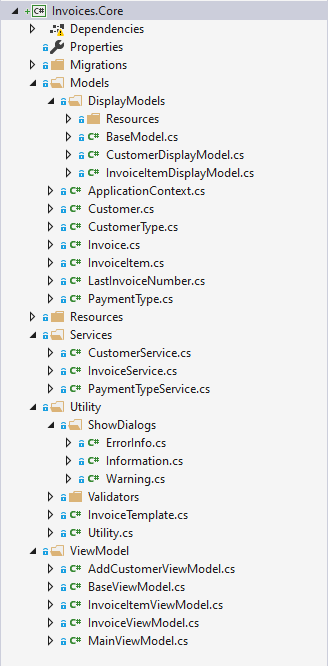
\includegraphics[width=0.5\linewidth]{Rysunki/core.png}
  \caption{Struktura projektu Core}
  \label{fig:Core}
\end{figure}

Z kolei w UI (rys. \ref{fig:UI}) widoki wyświetlane użytkownikowi.

\begin{figure}[ht!]
\centering
  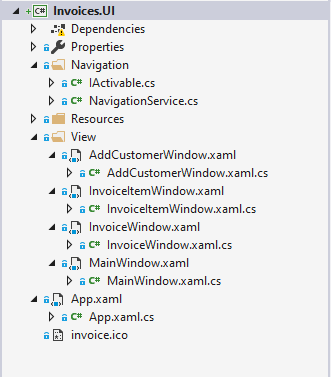
\includegraphics[width=0.5\linewidth]{Rysunki/ui.png}
  \caption{Struktura projektu UI}
  \label{fig:UI}
\end{figure}

\newpage ~\newpage
\section{Podstawowe obiekty aplikacji\label{AppObjects}}
Rysunek \ref{fig:classDiagram} przedstawia klasy znajdujące się w aplikacji. Wyróżniamy 3 główne klasy oraz 3 pomocnicze (w przyszłości mogą zostać rozbudowane). 

\begin{figure}[ht!]
  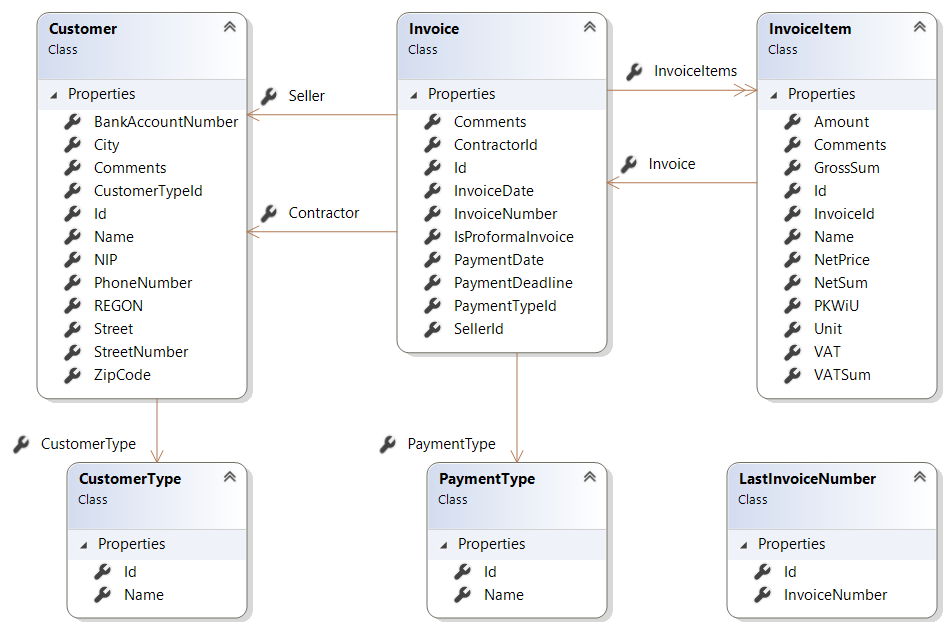
\includegraphics[width=\linewidth]{Rysunki/ClassDiagram.png}
  \caption{Diagram klas}
  \label{fig:classDiagram}
\end{figure}

\subsection{Customer}
Klasa Customer reprezentuje klienta aplikacji. Rozróżniamy dwa typy klientów: Kontrahent (osoba dla której wystawiamy fakturę) oraz Sprzedawca (osoba wystawiająca fakturę).
\\\\
Właściwości:
\begin{itemize}
    \item Name - imię i nazwisko klienta/firmy
    \item City - miasto, w którym klient urzęduje lub w którym znajduje się firma
    \item ZipCode - kod pocztowy
    \item Street - ulica, na której klient mieszka lub na której znajduje się firma
    \item StreetNumber - numer domu i mieszkania
    \item PhoneNumber - numer telefonu klienta/firmy
    \item NIP - Numer identyfikacji podatkowej
    \item REGON - (Rejestr Gospodarki Narodowej), Krajowy Rejestr Urzędowy Podmiotów Gospodarki Narodowej
    \item BankAccountNumber - numer konta bankowego klienta/firmy
    \item Comments - uwagi do klienta/firmy
    \item CustomerType - jest to instancja klasy CustomerType, która definiuje role klienta (Kontrahent, Sprzedawca)
    \item CustomerTypeId - pomocnicza zmienna pozwalająca w łatwy sposób odczytać typ klienta.
\end{itemize}

\subsection{Invoice}
Klasa Invoice reprezentuje faktury w aplikacji. Jest to najważniejsza klasa w całej aplikacji.
\\\\
Właściwości:
\begin{itemize}
    \item InvoiceNumber - numer faktury, ustalany na podstawie poprzedniego numeru faktury (format: kolejny numer/rok).
    \item InvoiceDate - data wystawienia faktury
    \item PaymentDeadline - ostateczny termin płatności za fakturę
    \item PaymentDate - data kiedy faktura została opłacona
    \item IsProformaInvoice - czy faktura jest fakturą pro forma
    \item Comments - uwagi do faktury
    \item Contractor - jest to instancja klasy Customer, która definiuje kto jest kontrahentem na fakturze
    \item Seller - jest to instancja klasy Customer, która definiuje kto jest sprzedawcą na fakturze
    \item PaymentType - jest to instancja klasy PaymentType, która definiuje metodę płatności za fakturę
    \item InvoiceItems - jest to kolekcja przedmiotów/produktów, które znajdują się na fakturze
    \item ContractorId oraz SellerId - dwie pomocnicze zmienne pozwalające w łatwy sposób odczytać klienta.
    \item PaymentTypeId - pomocnicza zmienna pozwalająca w łatwy sposób odczytać rodzaj płatności.
\end{itemize}

\subsection{InvoiceItem}
Klasa InvoiceItem reprezentuje przedmioty, które znajdują się na fakturze. Bez produktów faktura nie może zostać utworzona.
\\\\
Właściwości:
\begin{itemize}
    \item Name - nazwa produktu
    \item PKWiU - Polska Klasyfikacja Wyrobów i Usług
    \item Unit - jednostka w jakiej jest kupowany przedmiot (sztuki, opakowania, kilogramy)
    \item NetPrice - cena netto produktu
    \item Amount - ilość kupowanego produktu
    \item NetSum - suma netto kupowanego produktu, jest to cena netto pomnożona razy ilość kupowanego produktu
    \item VAT - podatek VAT podawany w procentach
    \item GrossSum - suma brutto kupowanego produktu, jest to suma netto pomnożona razy podatek VAT
    \item VATSum - suma podatku VAT, jest to różnica sumy brutto i sumy netto produktu
    \item Comments - uwagi do produktu
    \item Invoice - jest to instancja klasy Invoice, która ma na celu zidentyfikowanie do jakiej faktury należy dany produkt
    \item InvoiceId - pomocnicza zmienna pozwalająca odczytać fakturę
\end{itemize}

\subsection{CustomerType}
CustomerType to pomocnicza klasa pozwalająca zidentyfikować rodzaj klienta. Klasa ta posiada jedną właściwość jaką jest nazwa klienta (Kontrahent, Sprzedawca).

\subsection{PaymentType}
PaymentType to pomocnicza klasa pozwalająca zidentyfikować rodzaj płatności. Klasa ta posiada jedną właściwość jaką jest nazwa płatności (Gotówka, Przelew lub płatność kartą).

\subsection{LastInvoiceNumber}
LastInvoiceNumber to pomocnicza klasa pozwalająca na wygenerowanie nowego numeru porządkowego faktury. Posiada jedną właściwość jaką jest numer faktury (jest to ostatni numer faktury z danego roku). 

\section{Implementacja aplikacji} %Projekt przypadków użycia
Na poniższych rysunkach zostały przedstawione zależności pomiędzy pozostałymi klasami, widokami oraz modelami widoków w projekcie, a także metody, które znajdują się w poszczególnych klasach.

W aplikacji zostały utworzone dwie dodatkowe klasy DisplayModels, które ułatwiają wyświetlanie oraz wprowadzanie danych przez użytkownika. Obie te klasy dziedziczą po abstrakcyjnej klasie BaseModel. Klasa BaseModel implementuje 2 główne funkcje:

\begin{itemize}
    \item SetProperty<T> - metoda informuje widok, że nastąpiła zmiana w którejś z właściwości (użytkownik wprowadził zmianę)
    \item ValidateProperty<T> - metoda służy do sprawdzenia poprawności wpisanych danych przez użytkownika
\end{itemize}

Na rysunku \ref{fig:displayModelsDiagram} zostały przedstawione klasy CustomerDisplayModel i InvoiceItemDisplayModel, które posiadają takie same pola co klasy im odpowiadające (Customer oraz InvoiceItem). Jedyną różnicą jest to, że w klasach DisplayModels wszystkie pola są typu string.

\begin{figure}[ht!]
  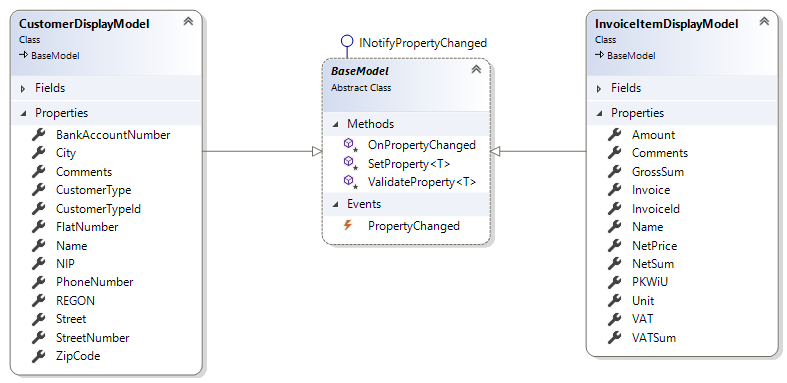
\includegraphics[width=\linewidth]{Rysunki/DisplayModelsDiagram.png}
  \caption{Diagram pomocniczych modeli}
  \label{fig:displayModelsDiagram}
\end{figure}

\subsection{AddCustomer}

\subsubsection{ViewModel}
Na rysunku \ref{fig:addCustomerViewModelDiagram} przedstawiony został, wraz ze związkami z innymi klasami, diagram widoku modelu dodawania klienta. 

\begin{figure}[ht!]
  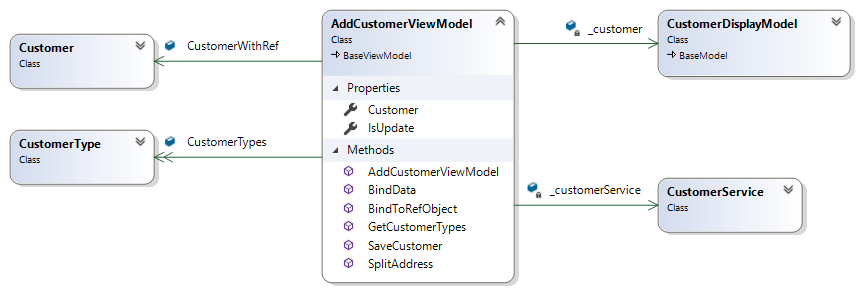
\includegraphics[width=\linewidth]{Rysunki/AddCustomerViewModelDiagram.png}
  \caption{Diagram modelu widoku dodawania klienta}
  \label{fig:addCustomerViewModelDiagram}
\end{figure}

Właściwość CustomerWithRef jest referencją przekazanego do view modelu obiektu, przez co później łatwiej edytować obiekty.
Atrybuty pola \_customer są związane z poszczególnymi kontrolkami na widoku AddCustomerWindow. Przez taki zabieg nie musimy się martwić o sczytywanie zawartości, ponieważ mamy je od razu w atrybutach obiektu \_customer. 
\\
W konstruktorze wstrzykiwana jest zależność \_customerService, przez co nie musimy się martwić przekazywaniem obiektu typu CustomerService, gdy tworzymy nową instancję AddCustomerViewModel. Metody BindData oraz BindToRefObject służą przygotowaniu wprowadzonych danych do zapisania. Metoda SplitAddress, dzieli otrzymany numer budynku oraz lokalu (są połączone) na dwie osobne wartości. 

Ważniejsze metody:

\begin{enumerate}
    \item \textbf{BindData} \\
    Metoda służy przypisaniu przychodzących danych do obiektu wyświetlanego na widoku. Przed każdym przypisaniem sprawdzane jest czy dana nie jest pusta. 
    \\
    \item \textbf{BindDataToRef} \\
    Metoda przypisuje obiekt wyświetlany na widoku do obiektu przekazanego poprzez referencję. 
    \\
    \item \textbf{SplitAddress} \\
    Metoda rozdziela numer na dwa osobne obiekty (numer budynku oraz numer lokalu). W bazie danych te dwa numery trzymane są jako jeden obiekt
\end{enumerate}

\subsubsection{View}
Klasa AddCustomerWindow (rysunek \ref{fig:addCustomerWindowDiagram}) implementuje interfejs IActivable, dzięki któremu jesteśmy w stanie przekazywać parametry do widoku. Posiada również pole ViewModel typu AddCustomerViewModel (konwencja MVVM).

\begin{figure}[ht!]
\centering
  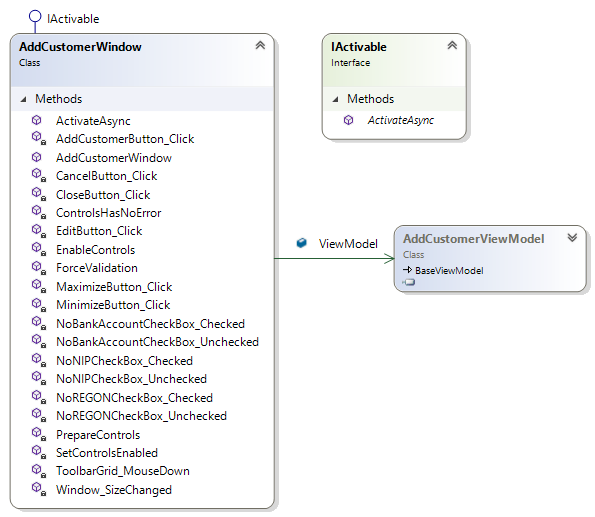
\includegraphics[width=0.7\linewidth]{Rysunki/AddCustomerWindowDiagram.png}
  \caption{Diagram klasy widoku dodawania klienta}
  \label{fig:addCustomerWindowDiagram}
\end{figure}

Ważniejsze metody:

\begin{enumerate}
    \item \textbf{ActivateAsync} \\
    Metoda jest zaimplementowana z interfejsu \textbf{IActivable} i wywoływana przed pokazaniem widoku. Funkcja przyjmuje parametr, dzięki czemu jesteśmy w stanie przekazać dowolny obiekt do naszego widoku. W metodzie zostaje przygotowany obiekt (przypisanie danych do obiektu, wypełnienie kontrolek odpowiednimi danymi), który zostanie wyświetlony w oknie, dlatego ważnym jest, żeby metoda uruchomiła się przed załadowaniem widoku. 
    \\
    \item \textbf{AddCustomerButton\_Click} \\
    Jest to jedna z ważniejszych metod w widoku. Wywoływana jest kliknięciem w przycisk i zapisuje obiekt Customer w bazie danych. Funkcja sprawdza na początku czy wszystkie dane zostały wprowadzone prawidłowo (jeżeli nie, dostajemy stosowny komunikat). Następnie wszystkie dane zostają przypisane do obiektu z referencją i obiekt zapisywany jest w bazie danych.
    \\
    \item \textbf{ForceValidation} \\
    Metoda niejawnie aktualizuje kontrolki. Po takim zabiegu jeżeli jakaś kontrolka nie została uzupełniona lub została uzupełniona błędnie otrzymamy stosowny komunikat (nie będziemy też w stanie zapisać obiektu Customer).
\end{enumerate}


\subsubsection{Service}
CustomerService odpowiada za połączenie z bazą danych a także operacje CRUD (Create, Read, Update, Delete). Na listingu \ref{list:CustomerSUD} zostały przedstawione metody do zapisu, zaktualizowania oraz usunięcia obiektu Customer.

\begin{lstlisting}[language={[Sharp]C},label=list:CustomerSUD,caption=Przykładowe metody w serwisie CustomerService, basicstyle=\footnotesize\ttfamily]
public void SaveCustomer(Customer customerWithRef)
{
    _ctx.Customers.Add(customerWithRef);
    _ctx.SaveChanges();
}

public void UpdateCustomer(Customer customerWithRef)
{
    var oldCustomer = _ctx.Customers.Find(customerWithRef.Id);

    _ctx.Entry(oldCustomer).CurrentValues.SetValues(customerWithRef);
    _ctx.SaveChanges();
}

public void DeleteCustomer(Customer customer)
{
    _ctx.Customers.Remove(customer);
    _ctx.SaveChanges();
}
\end{lstlisting}

Wszystkie zapytania do bazy realizowane są za pomocą Entity Framework Core. 

\subsection{Invoice}

\subsubsection{ViewModel}
Na rysunku \ref{fig:InvoiceViewModelDiagram} przedstawiony został diagram klasy InvoiceViewModel. 

\begin{figure}[ht!]
  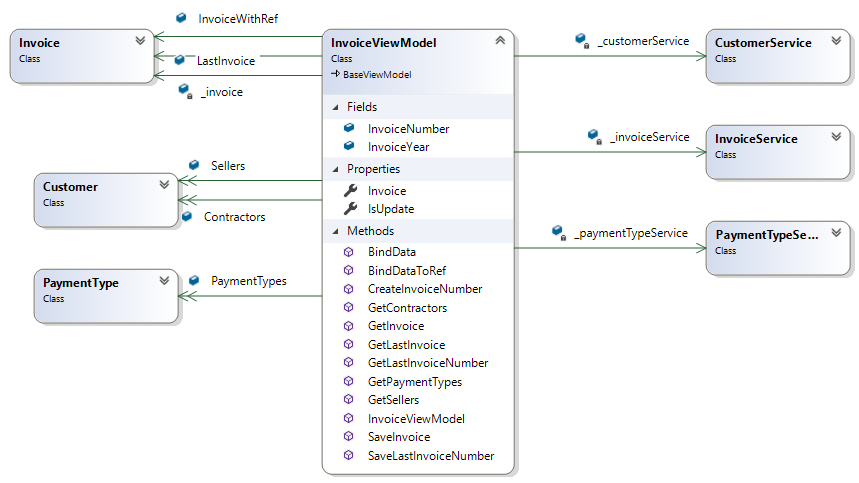
\includegraphics[width=\linewidth]{Rysunki/InvoiceViewModelDiagram.png}
  \caption{Diagram modelu widoku faktur}
  \label{fig:InvoiceViewModelDiagram}
\end{figure}

Obiekt InvoiceWithRef trzyma referencję do oryginalnego obiektu faktury (potrzebne przy aktualizacji faktur). LastInvoice jest ostatnią fakturą dodaną do bazy danych. Jest potrzebna w celu ustalenia kolejnego numeru porządkowego faktury. Właściwość Invoice została utworzona w celu wyświetlenia oraz późniejszego sczytania wartości z widoku. Do InvoiceViewModel zostają wstrzyknięte 3 serwisy które dostarczają oraz pozwalają zapisać nasze dane w bazie. Klasa InvoiceViewModel posiada także dwa obiekty typu Customer, które identyfikują kontrahenta oraz sprzedawcę. Model widoku posiada również 3 kolekcje, które oznaczone są na diagramie przez podwójną strzałkę. Listy dostarczają nam wszystkich kontrahentów oraz sprzedawców, a także typy płatności za faktury.

Ważniejsze metody:
\begin{enumerate}
    \item \textbf{BindData oraz BindDataToRef} - metody bardzo podobne do opisanych wcześniej (przy AddCustomer), służą do przypisania przychodzących oraz wychodzących danych.
    \item \textbf{CreateInvoiceNumber} \\
    Metoda generuje kolejny numer porządkowy (na podstawie ostatniej faktury) przy tworzeniu nowej faktury. Jako parametr metody jest przekazywany ostatni numer porządkowy. W przypadku, gdy rok jest ten sam liczba zwiększa się o jeden, gdy rozpoczyna się nowy rok, numeracja startuje od początku i rok jest aktualizowany.
\end{enumerate}

\subsubsection{View}
Na rysunku \ref{fig:InvoiceWindowDiagram} został przedstawiony diagram klasy widoku faktur. Klasa implementuje interfejs IActivable. Interfejs ten dostarcza nam metodę \textbf{ActivateAsync}, która przyjmuje parametr, dzięki czemu jesteśmy w stanie przekazać obiekt do naszego widoku. Klasa posiada dwa obiekty. Pierwszy z nich to InvoiceViewModel, w którym jest zaimplementowana cała logika. Drugi to NavigationService, który pozwala uruchomić kolejne okna z zachowaniem dependency injection. 

\newpage
\begin{figure}[ht!]
\centering
  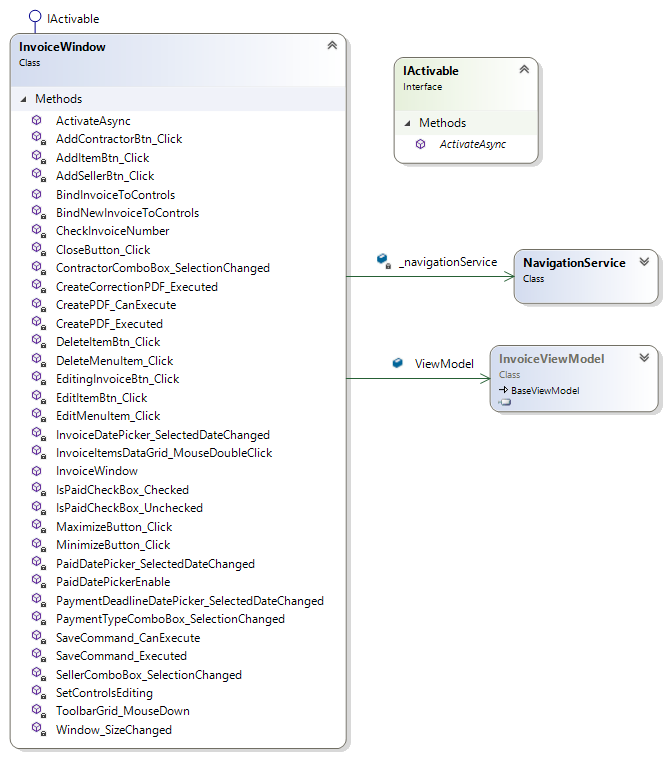
\includegraphics[width=0.7\linewidth]{Rysunki/InvoiceWindowDiagram.png}
  \caption{Diagram widoku faktur}
  \label{fig:InvoiceWindowDiagram}
\end{figure}

Ważniejsze metody:
\begin{enumerate}
    \item \textbf{AddContractorBtn\_Click} i \textbf{AddSellerBtn\_Click} \\
    Metoda uruchamia widok, w którym możemy dodać nowego kontrahenta, bądź sprzedawcę. Funkcja korzysta z zależności NavigationService w celu poprawnego uruchomienia okna. Przed dodaniem sprawdzane jest czy obiekt nie jest pusty.
    \item \textbf{AddItemBtn\_Click} \\
    Funckja pozwala na dodanie nowej pozycji na fakturze. Zostaje uruchomione nowe okno (InvoiceItemWindow), w którym dodajemy pozycję na fakturę.
    \item \textbf{BindInvoiceToControls} \\
    Metoda przypisuje odpowiednie właściwości obiektu Invoice to kontrolek, które wyświetlane są na widoku. Funkcja jest uruchamiana w trakcie edycji faktury i ma swój odpowiednik w przypadku tworzenia nowej faktury.
    \item \textbf{BindNewInvoiceToControls} \\
    Funkcja działa tak jak wyżej tylko uruchamiana jest przy tworzeniu nowej faktury.
    \item \textbf{CheckInvoiceNumber} \\
    Metoda sprawdza poprawność utworzonego numeru porządkowego faktury. Tworzy też nowy numer porządkowy w przypadku ustawienia daty wystawienia faktury na kolejny rok.
    \item \textbf{CreatePDF\_Executed} i \textbf{CreateCorrectionPDF\_Executed} \\
    Metody tworzą kolejno plik PDF z wybraną przez użytkownika fakturą oraz korektę do faktury (jeżeli na fakturze pojawiły się jakieś zmiany). 
    \item \textbf{DeleteItemBtn\_Click} i \textbf{DeleteMenuItem\_Click} \\
    Obie metody pozwalają na usunięcie pozycji z faktury, w przypadku niezaznaczenia produktu, aplikacja wyświetla stosowny komunikat. 
    \item \textbf{EditItemBtn\_Click}, \textbf{EditMenuItem\_Click} oraz \\
    \textbf{InvoiceItemsDataGrid\_MouseDoubleClick} \\
    Obie metody pozwalają na edytowanie pozycji z faktury, w przypadku niezaznaczenia produktu, aplikacja wyświetla stosowny komunikat. 
    \item \textbf{SaveCommand\_Executed} \\
    Metoda na początku sprawdza czy kontrahent oraz sprzedawca zostali wybrani prawidłowo (oraz czy w ogóle zostali wybrani). Następnie przypisuje wszystkie właściwości do obiektu z referencją i zapisuje fakturę w bazie.
\end{enumerate}

Metody z dopiskiem \textbf{\_SelectedDateChanged} sprawdzają czy wszystkie daty na fakturze zostały wprowadzone prawidłowo. W przypadku podania złych dat aplikacja wyświetla odpowiedni komunikat. 

\subsubsection{Service}
Na listingu \ref{list:InvoiceService} zostały przedstawione przykładowe metody operacji CRUD. 

\begin{lstlisting}[language={[Sharp]C},label=list:InvoiceService,caption=Przykładowe metody w serwisie InvoiceService, basicstyle=\footnotesize\ttfamily]
public List<Invoice> GetInvoices()
{
    return _ctx.Invoices
        .Include(p => p.InvoiceItems)
        .Include(seller => seller.Seller)
        .Include(contractor => contractor.Contractor)
        .Include(paymentType => paymentType.PaymentType)
        .ToList();
}

public Invoice GetInvoice(int id)
{
    return _ctx.Invoices
        .Include(x => x.PaymentType)
        .Include(x => x.InvoiceItems)
        .Include(x => x.Contractor)
        .Include(x => x.Seller)
        .FirstOrDefault(x => x.Id == id);
}

public void DeleteInvoice(Invoice invoice)
{
    _ctx.Invoices.Remove(invoice);
    _ctx.SaveChanges();
}

public void SaveInvoice(Invoice invoice)
{
    _ctx.Invoices.Add(invoice);
    _ctx.SaveChanges();
}

public void UpdateInvoice(Invoice invoice)
{
    var oldInvoice = _ctx.Invoices.Find(invoice.Id);

    _ctx.Entry(oldInvoice).CurrentValues.SetValues(invoice);
    _ctx.SaveChanges();
}
\end{lstlisting}

Pierwsza z metod \textbf{GetInvoices} pobiera z bazy danych listę wszystkich faktur i dołącza do nich odpowiadające im obiekty InvoiceItems, Customer oraz PaymentType za pomocą funkcji \textbf{Include} dostarczanej przez Entity Framework Core. 

\subsection{InvoiceItem}
\subsubsection{ViewModel}
Na rysunku \ref{fig:InvoiceItemDiagram} został przedstawiony diagram klasy InvoiceItemViewModel. Klasa ta posiada 2 główne obiekty (podobnie jak pozostałem klasy ViewModel):

\begin{enumerate}
    \item InvoiceItem (typu InvoiceItemDisplayModel) - obiekt wyświetlany oraz bindowany do widoku
    \item InvoiceItemWithRef (typu InvoiceItem) - obiekt z referencją, zapisywany do bazy danych
\end{enumerate}

\begin{figure}[ht!]
  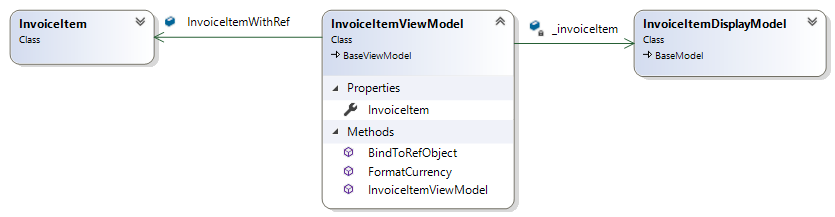
\includegraphics[width=\linewidth]{Rysunki/InvoiceItemViewModelDiagram.png}
  \caption{Diagram modelu widoku InvoiceItem}
  \label{fig:InvoiceItemDiagram}
\end{figure}

InvoiceItemViewModel posiada dwie ważne metody:

\begin{enumerate}
    \item \textbf{BindToRefObject} \\
    Tak jak w pozostałych modelach widoku, w metodzie zostają przypisane wartości, wprowadzone przez użytkownika, z obiektu InvoiceItem do obiektu z referencją InvoiceItemWithRef. 
    \item \textbf{FormatCurrency} \\
    Metoda została utworzona w celu poprawnej konwersji waluty na format polski.
\end{enumerate}

\subsubsection{View}
Na rysunku \ref{fig:InvoiceItemWindowDiagram} został przedstawiony diagram klasy widoku pozycji z faktury. Klasa implementuje interfejs IActivable. Klasa posiada jeden główny obiekt InvoiceItemViewModel, który implementuje cała logikę widoku.

\newpage
\begin{figure}[ht!]
\centering
  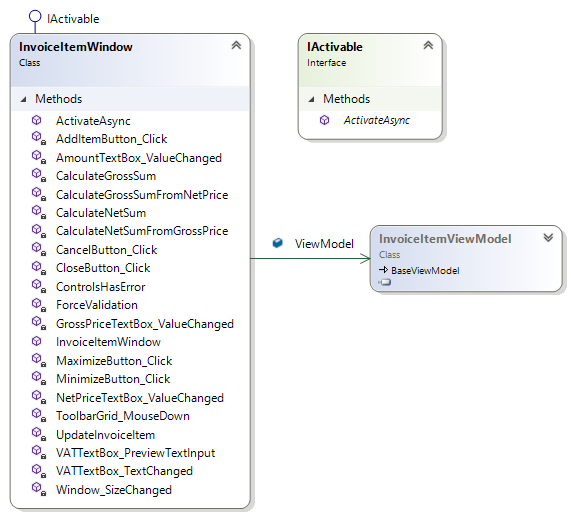
\includegraphics[width=0.7\linewidth]{Rysunki/InvoiceItemWindowDiagram.png}
  \caption{Diagram widoku modelu InvoiceItem}
  \label{fig:InvoiceItemWindowDiagram}
\end{figure}

Ważniejsze metody:
\begin{enumerate}
    \item \textbf{ActivateAsync} \\
    Metoda została zaimplementowana z interfejsu \textbf{IActivable}. Funkcja pozwala nam na przekazanie dowolnego obiektu do naszego widoku. Następnie w metodzie obiekt zostaje przygotowany i podpięty do kontrolek, by później móc zostać poprawnie wyświetlony. 
    \item \textbf{AddItemButton\_Click}\\
    Jest to najważniejsza metoda w widoku. Wywoływana jest poprzez kliknięcie przycisku zapisywania pozycji. Funkcja sprawdza na początku czy wszystkie dane zostały wpisane prawidłowo. Jeżeli dane zostały wprowadzone źle aplikacja informuje nas komunikatem, w przeciwnym razie pozycja zostaje dodana do faktury.
    \item \textbf{ForceValidation} i \textbf{ControlsHasNoError} \\
    Obie metody służą do walidacji wpisanych przez użytkownika danych. Pierwsza z nich niejawnie aktualizuje kontrolkę w celu wywołania walidacji, z kolei druga sprawdza czy, na którejś kontrolce, wystąpił błąd walidacji.
\end{enumerate}

Funkcje z dopiskiem \textbf{\_ValueChanged} oraz \textbf{\_TextChanged} na bieżąco obliczają wartości: 
\begin{itemize}
    \item Ceny netto
    \item Ceny brutto
    \item Sumy netto
    \item Sumy brutto
    \item Sumy VAT
\end{itemize}

\subsubsection{Service}
W przypadku InvoiceItem serwis nie został utworzony, ponieważ nie było takiej potrzeby. Wszystkie zapytania związane z dodawaniem, usuwaniem i czytaniem pozycji z faktury realizowane są automatycznie przy dodawaniu nowego/edycji obiektu Invoice.

\subsection{Main}

\subsubsection{ViewModel}
Rysunek \ref{fig:MainViewModelDiagram} przedstawia diagram widoku modelu MainViewModel. ViewModel posiada 3 główne kolekcje, które dostarczają dane do naszego widoku. Do MainViewModel zostały wstrzyknięte 2 serwisy: InvoiceService (pobiera dane faktur z bazy) i CustomerService (pobiera dane kontrahentów oraz sprzedawców z bazy). Widok modelu nie posiada skomplikowanych funkcji, ponieważ został stworzony tylko do wyświetlania oraz usuwania danych. \\
Ważniejszą metodą jest \textbf{DeleteInvoice}. Funkcja nie tylko usuwa wybraną przez użytkownika fakturę, ale także zmienia kolejny numer porządkowy faktury. Numeracja faktur musi odbywać się po kolei i powinna być ciągła.

\begin{figure}[ht!]
  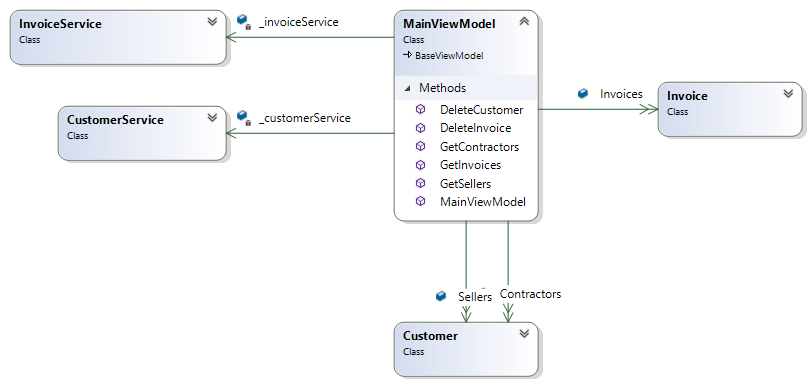
\includegraphics[width=\linewidth]{Rysunki/MainViewModelDiagram.png}
  \caption{Diagram głównego modelu widoku}
  \label{fig:MainViewModelDiagram}
\end{figure}

\subsubsection{View}
Na rysunku \ref{fig:MainWindowDiagram} został przedstawiony diagram głównego widoku aplikacji. MainWindow ma wstrzyknięte 2 zależności: NavigationService (służący do otwierania kolejnych widoków) i MainViewModel (widok modelu). 
\\
Ważniejsze metody:
\begin{enumerate}
    \item \textbf{AddContractorButton\_Click} i \textbf{AddSellerButton\_Click} \\
    Metoda otwiera asynchroniczny widok (AddCustomer), który umożliwia dodanie nowego sprzedawcy lub kontrahenta, w zależności od wybranego typu.
    \item \textbf{AddInvoiceButton\_Click} \\
    Funkcja otwiera asynchroniczny widok (Invoice), pozwalający na dodanie nowej faktury.
    \item \textbf{SearchInvoiceTextBox\_KeyUp} \\
    Metoda służy do wyszukiwania faktur. Faktury można wyszukać po: numerze faktury, nazwie (kontrahenta, sprzedawcy), ulicy i mieście (kontrahenta) oraz dacie wystawienia.
    \item \textbf{SearchSellerTextBox\_KeyUp} i \textbf{SearchContractorTextBox\_KeyUp} \\
    Metody służą do wyszukania sprzedawcy/kontrahenta. Osoby te możemy wyszukać po: nazwie, NIPie, REGONie, ulicy oraz mieście.
\end{enumerate}

Metody z dopiskiem \textbf{\_MouseDoubleClick} służą do edytowania faktury, kontrahenta i sprzedawcy. Funkcja wywołuje się podczas dwukrotnego kliknięcia w pozycję na liście.

\begin{figure}[ht!]
\centering
  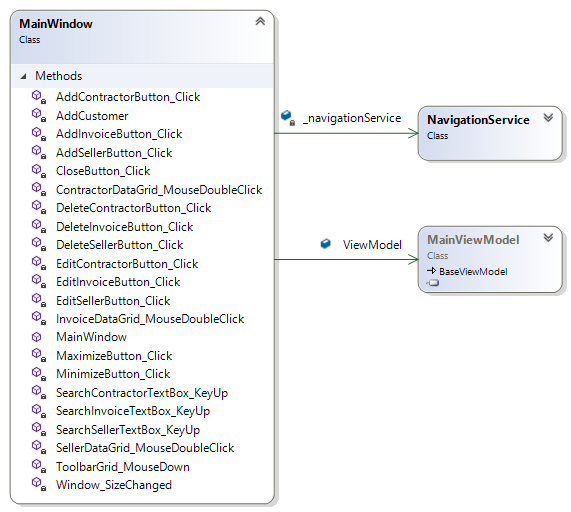
\includegraphics[width=0.7\linewidth]{Rysunki/MainWindowDiagram.png}
  \caption{Diagram głównego widoku}
  \label{fig:MainWindowDiagram}
\end{figure}

\subsubsection{Service}

W przypadku Main serwis nie został utworzony. Widok główny korzysta z serwisów \textbf{InvoiceService} oraz \textbf{CustomerService}, które dostarczają wszystkie potrzebne funkcje.

\subsection{NavigationService}
Na listingu \ref{list:NavigationService} został przedstawiony serwis służący do nawigacji między widokami (uruchamianie okien). NavigationService musiał zostać zaimplementowany z powodu Dependency Injection w projekcie. W przeciwnym razie nie bylibyśmy w stanie otwierać widoków ze wstrzykniętymi zależnościami.

\begin{lstlisting}[language={[Sharp]C},label=list:NavigationService,caption=Serwis do nawigacji między widokami, basicstyle=\footnotesize\ttfamily]
private readonly IServiceProvider _serviceProvider;

public NavigationService(IServiceProvider serviceProvider)
{
    _serviceProvider = serviceProvider;
}

public async Task ShowAsync<T>(object parameter = null) where T : Window
{
    var window = _serviceProvider.GetRequiredService<T>();
    if (window is IActivable activableWindow)
    {
        await activableWindow.ActivateAsync(parameter);
    }

    window.Show();
}

public async Task<bool?> ShowDialogAsync<T>(object parameter = null) where T : Window
{
    var window = _serviceProvider.GetRequiredService<T>();
    if (window is IActivable activableWindow)
    {
        await activableWindow.ActivateAsync(parameter);
    }

    return window.ShowDialog();
}
\end{lstlisting}

\subsection{InvoiceTemplate}
InvoiceTemplate jest jedną z głównych klas w projekcie. Odpowiada za generowanie pliku PDF z przekazanej jako parametr faktury. Na rysunku \ref{fig:InvoiceTemplateDiagram} został przedstawiony diagram klasy wraz ze wszystkimi polami i metodami. Zostało utworzonych kilka podstawowych czcionek o różnych parametrach (wielkość, pogrubienie). W klasie szablonu zostało dodane pole typu Invoice, z którego odczytujemy wszystkie informacje potrzebne do utworzenia faktury. 

\begin{figure}[ht!]
\centering
  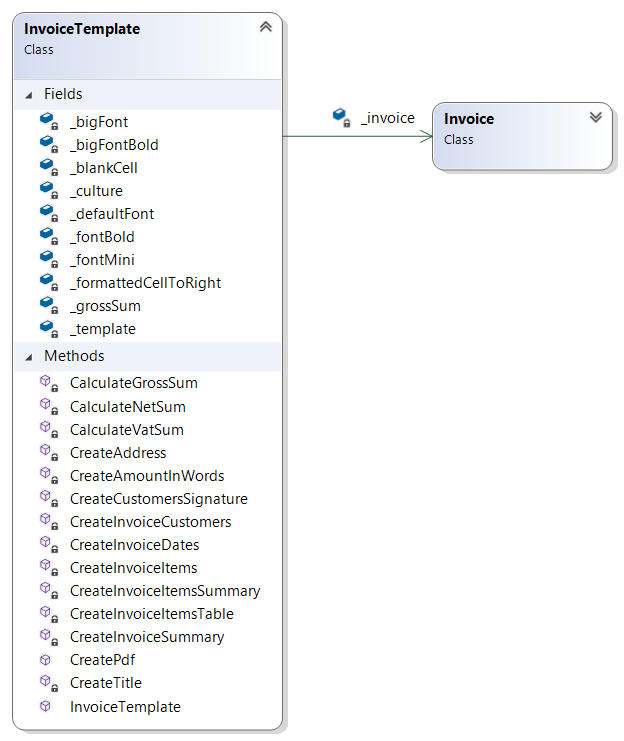
\includegraphics[width=0.6\linewidth]{Rysunki/InvoiceTemplate.png}
  \caption{Diagram klasy szablonu faktury}
  \label{fig:InvoiceTemplateDiagram}
\end{figure}

Główna metoda \textbf{CreatePdf} łączy wszystkie metody i generuje cały plik PDF.

\begin{lstlisting}[language={[Sharp]C},label=list:createPDF,caption=Metoda CreatePDF, basicstyle=\footnotesize\ttfamily]
public string CreatePdf(Utility.InvoiceTemplateStruct template)
{
    Document document = new Document(PageSize.A4, 50, 50, 70, 10);
    PdfWriter.GetInstance(document, new FileStream(file, FileMode.Create));

    document.Open();

    //create invoice title
    document.Add(_template.InvoiceType == Utility.InvoiceTypeTemplateEnum.Original
        ? CreateTitle("Oryginał", invoiceTitle)
        : CreateTitle("Kopia", invoiceTitle));


    document.Add(newLine);

    //create invoice date, invoice number and city
    document.Add(CreateInvoiceDates());

    document.Add(newLine);

    //create seller and contractor information
    document.Add(CreateInvoiceCustomers());

    document.Add(newLine);

    //create invoice items
    document.Add(CreateInvoiceItemsTable());

    document.Add(CreateInvoiceItems(_invoice.InvoiceItems.ToList()));

    document.Add(CreateInvoiceItemsSummary());

    document.Add(newLine);

    document.Add(CreateInvoiceSummary());

    for (int i = 0; i < 8; i++)
    {
        document.Add(newLine);
    }

    document.Add(CreateCustomersSignature());

    document.Close();

    return file;
}
\end{lstlisting}

Szablon generuje plik PDF na podstawie tworzenia tabel, które potem wypełniamy komórkami z danymi. Wszystkie metody w szablonie zwracają utworzoną tabelę, która dodawana jest do dokumentu za pomocą polecenia \textit{document.Add()}. W listingu \ref{list:createPDF} zostało pokazane złożenie wszystkich metod, które po kolei generują cały plik: 

\begin{enumerate}
    \item \textbf{CreateTitle} - utworzenie tytułu faktury (Faktura VAT, Faktura PRO FORMA lub korekta do faktury VAT) oraz dodanie czy faktura jest oryginałem czy kopią
    \item \textbf{CreateInvoiceDates} - utworzenie tabeli zawierającej daty sprzedaży i wystawienia faktury, miejsce wystawienia oraz numer faktury
    \item \textbf{CreateInvoiceCustomers} - dodanie do faktury danych sprzedawcy oraz nabywcy
    \item \textbf{CreateInvoiceItemsTable} - utworzenie tabeli dla pozycji z faktury
    \item \textbf{CreateInvoiceItems} - wypełnienie tabeli wszystkimi pozycjami znajdującymi się na fakturze
    \item \textbf{CreateInvoiceItemsSummary} - utworzenie podsumowania wszystkich pozycji (wyliczona suma netto, brutto oraz VAT)
    \item \textbf{CreateInvoiceSummary} - wygenerowanie podsumowania dla faktury (suma brutto liczbą oraz słownie, forma płatności, czy zapłacono, termin płatności, numer konta bankowego sprzedawcy oraz uwagi do faktury)
    \item \textbf{CreateCustomersSignature} - utworzenie miejsca na podpisy osób odpowiedzialnych za odbiór oraz wystawienie faktury
\end{enumerate}

Metody wyglądają podobnie. Tabele, które zwracają funkcje, różnią się jedynie układem oraz danymi. Przykładowa metoda:

\begin{lstlisting}[language={[Sharp]C},label=list:createTitle,caption=Metoda CreateTitle, basicstyle=\footnotesize\ttfamily]
private IElement CreateTitle(string invoiceType, string invoiceTitle)
{
    PdfPTable table = new PdfPTable(1);

    int[] colWidth = { 100 };
    table.SetWidths(colWidth);
    table.WidthPercentage = 100;

    PdfPCell invoiceTitleCell = new PdfPCell(new Phrase(invoiceTitle, _bigFontBold))
    {
        VerticalAlignment = Element.ALIGN_MIDDLE,
        HorizontalAlignment = Element.ALIGN_CENTER,
        Padding = 2,
        Border = 0
    };
    table.AddCell(invoiceTitleCell);
    PdfPCell invoiceTypeCell = new PdfPCell(new Phrase(invoiceType, _bigFont))
    {
        VerticalAlignment = Element.ALIGN_MIDDLE,
        HorizontalAlignment = Element.ALIGN_CENTER,
        Padding = 2,
        Border = 0
    };
    table.AddCell(invoiceTypeCell);

    return table;
}
\end{lstlisting}

W listingu \ref{list:createTitle} tworzona jest tabela z jedną kolumną o szerokości 100. Następnie są dodane do niej dwie komórki, które są wycentrowane w pionie i poziomie. Po każdym utworzeniu są dodawane do tabeli. Na koniec funkcja zwraca utworzoną tabelę, która dodawana jest do dokumentu.

\section{Projekt bazy danych}

Rysunek \ref{fig:erdDiagram} przedstawia diagram ERD bazy danych wraz z zależnościami między encjami. Kolejny diagram \ref{fig:erdDiagramForeign} został uzupełniony o klucze obce. Została pokazana także relacja między encjami oraz kluczami. Ostatni rysunek \ref{fig:erdDiagramAttr} został uzupełniony pozostałymi atrybutami encji.

\begin{figure}[ht!]
\centering
  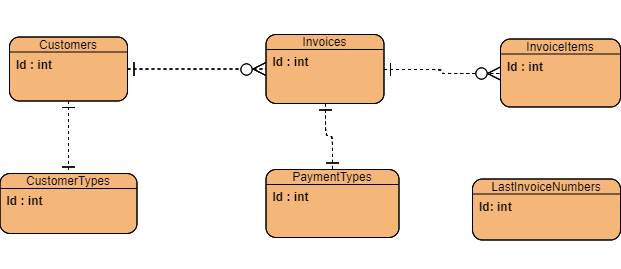
\includegraphics[width=0.7\linewidth]{Rysunki/ERD.png}
  \caption{Diagram ERD w notacji Martina}
  \label{fig:erdDiagram}
\end{figure}

\begin{figure}[ht!]
\centering
  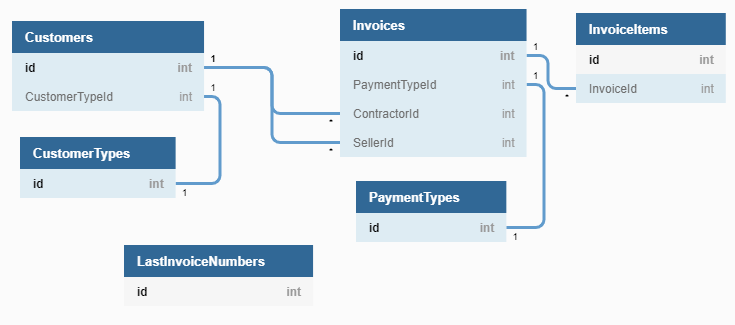
\includegraphics[width=0.8\linewidth]{Rysunki/ERD-relacje.png}
  \caption{Diagram ERD uzupełniony o klucze obce}
  \label{fig:erdDiagramForeign}
\end{figure}

\begin{figure}[ht!]
  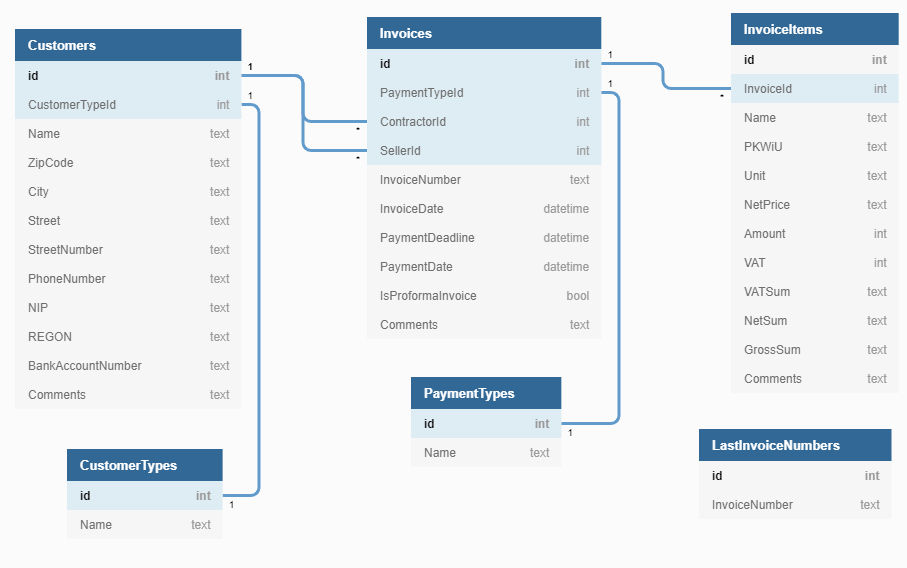
\includegraphics[width=\linewidth]{Rysunki/ERDAttr.png}
  \caption{Diagram ERD ze wszystkimi atrybutami encji}
  \label{fig:erdDiagramAttr}
\end{figure}

\newpage
Opcjonalność encji:

\begin{itemize}
    \item Każda faktura (Invoices) \textbf{musi} posiadać jednego sprzedawcę i jednego kontrahenta (Customers)
    \item Każda faktura \textbf{może} posiadać produkty/elementy (InvoicesItems)
    \item Każdy element/produkt (InvoiceItems) \textbf{musi} znajdować się na fakturze (Invoices)
    \item Każdy klient (Customers) \textbf{musi} mieć zdefiniowany typ
    (CustomerTypes)
    \item Każda faktura \textbf{musi} mieć zdefiniowany typ płatności (PaymentTypes)
\end{itemize}

W tabelach \ref{tab:CustomerAttr}, \ref{tab:InvoicesAttr} i \ref{tab:InvoiceItemsAttr} zostały przedstawione wszystkie atrybuty jakie posiadają kolejno encje Customers, Invoices oraz InvoiceItems. Każdy atrybut posiada swój typ oraz krótki opis.

\begin{table}[ht!]
\centering
\resizebox{0.9\textwidth}{!}{%
\begin{tabular}{|l|l|l|}
\hline
\textbf{Atrybut}  & \textbf{Typ}                                                       & \textbf{Opis}                                                                                                                             \\ \hline
Id                & \begin{tabular}[c]{@{}l@{}}INTEGER, \\ auto increment\end{tabular} & Klucz główny, unikalny, identyfikacja klienta                                                                                             \\ \hline
CustomerTypeId    & INTEGER                                                            & Klucz obcy, relacja z encją CustomerTypes                                                                                                 \\ \hline
Name              & TEXT                                                               & Nazwa firmy/klienta,                                                                                                                      \\ \hline
ZipCode           & TEXT                                                               & \begin{tabular}[c]{@{}l@{}}Kod pocztowy miasta, w którym znajduje się firma/\\ mieszka klient\end{tabular}                                \\ \hline
City              & TEXT                                                               & \begin{tabular}[c]{@{}l@{}}Nazwa miasta, w którym znajduje się firma/\\ mieszka klient\end{tabular}                                       \\ \hline
Street            & TEXT                                                               & \begin{tabular}[c]{@{}l@{}}Nazwa ulicy, na której znajduje się firma/\\ mieszka klient\end{tabular}                                       \\ \hline
StreetNumber      & TEXT                                                               & Numer budynku oraz numer lokalu                                                                                                           \\ \hline
PhoneNumber       & TEXT                                                               & Numer telefonu do firmy/klienta                                                                                                           \\ \hline
NIP               & TEXT                                                               & \begin{tabular}[c]{@{}l@{}}Numer identyfikacji podatkowej, \\ w formacie \#\#\#-\#\#\#-\#\#-\#\#\end{tabular}                             \\ \hline
REGON             & TEXT                                                               & \begin{tabular}[c]{@{}l@{}}numer identyfikacyjny REGON, \\ Rejestr Gospodarki Narodowej, \\ w formacie \#\#\#-\#\#-\#\#-\#\#\end{tabular} \\ \hline
BankAccountNumber & TEXT                                                               & Numer rachunku bankowego (26 cyfr)                                                                                                        \\ \hline
Comments          & TEXT                                                               & Uwagi do firmy/klienta                                                                                                                    \\ \hline
\end{tabular}%
}
\caption{Atrybuty encji Customers}
\label{tab:CustomerAttr}
\end{table}

\begin{table}[ht!]
\centering
\resizebox{0.9\textwidth}{!}{%
\begin{tabular}{|l|l|l|}
\hline
\textbf{Atrybut}  & \textbf{Typ}                                                      & \textbf{Opis}                                                                                                                        \\ \hline
Id                & \begin{tabular}[c]{@{}l@{}}INTEGER,\\ auto increment\end{tabular} & \begin{tabular}[c]{@{}l@{}}Klucz główny, unikalny, \\ identyfikacja faktury\end{tabular}                                             \\ \hline
ContractorId      & INTEGER                                                           & Klucz obcy encji Customers                                                                                                           \\ \hline
SellerId          & INTEGER                                                           & Klucz obcy encji Customers                                                                                                           \\ \hline
PaymentTypeId     & INTEGER                                                           & Klucz obcy encji PaymentTypes                                                                                                        \\ \hline
InvoiceNumber     & TEXT, unique                                                      & \begin{tabular}[c]{@{}l@{}}Numer porządkowy faktury, jest unikalny, \\ format (kolejne liczby całkowite)/(aktualny rok)\end{tabular} \\ \hline
InvoiceDate       & TEXT                                                              & Data wystawienia faktury                                                                                                             \\ \hline
PaymentDeadline   & TEXT                                                              & Termin płatności za fakturę                                                                                                          \\ \hline
PaymentDate       & TEXT                                                              & Data płatności za fakturę                                                                                                            \\ \hline
IsProformaInvoice & INTEGER                                                           & \begin{tabular}[c]{@{}l@{}}Wartość binarna określająca czy faktura \\ jest fakturą pro forma, czy fakturą VAT\end{tabular}           \\ \hline
Comments          & TEXT                                                              & Uwagi do faktury                                                                                                                     \\ \hline
\end{tabular}%
}
\caption{Atrybuty encji Invoices}
\label{tab:InvoicesAttr}
\end{table}


\begin{table}[ht!]
\centering
\resizebox{0.8\textwidth}{!}{%
\begin{tabular}{|l|l|l|}
\hline
\textbf{Atrybut} & \textbf{Typ}                                                      & \textbf{Opis}                                                                                    \\ \hline
Id               & \begin{tabular}[c]{@{}l@{}}INTEGER,\\ auto increment\end{tabular} & \begin{tabular}[c]{@{}l@{}}Klucz główny, unikalny,\\ identyfikacja pozycji faktury\end{tabular}  \\ \hline
InvoiceId        & INTEGER                                                           & Klucz obcy encji Invoices                                                                        \\ \hline
Name             & TEXT                                                              & Nazwa pozycji                                                                                    \\ \hline
PKWiU            & TEXT                                                              & Polska Klasyfikacja Wyrobów i Usług                                                              \\ \hline
Unit             & TEXT                                                              & \begin{tabular}[c]{@{}l@{}}jednostka w jakiej jest zapisywana\\ pozycja na fakturze\end{tabular} \\ \hline
NetPrice         & TEXT                                                              & Cena netto pozycji                                                                               \\ \hline
Amount           & INTEGER                                                           & Ilość w jakiej kupujemy pozycję                                                                  \\ \hline
VAT              & INTEGER                                                           & Podatek VAT, podawany w procentach                                                               \\ \hline
NetSum           & TEXT                                                              & Suma netto pozycji                                                                               \\ \hline
GrossSum         & TEXT                                                              & Suma brutto pozycji                                                                              \\ \hline
VATSum           & TEXT                                                              & Różnica sumy brutto i netto                                                                      \\ \hline
Comments         & TEXT                                                              & Uwagi do pozycji                                                                                 \\ \hline
\end{tabular}%
}
\caption{Atrybuty encji InvoiceItems}
\label{tab:InvoiceItemsAttr}
\end{table}

\newpage
W tabeli \ref{tab:entityRelations} przedstawiono relacje pomiędzy encjami. Encja Customers oraz Invoices połączone są relacją jeden do wielu, ponieważ każda faktura (Invoices) może posiadać jednego sprzedawcę i kontrahenta (Customers), a kontrahent oraz sprzedawca może znajdować się na wielu fakturach. Encja Invoices i InvoiceItems również jest połączona w relacji jeden do wielu. Każda faktura może mieć wiele produktów (InvoiceItems). Encje Customers i Invoices są w relacji 1:1 kolejno z encjami CustomerTypes (definiującej typ klienta - Sprzedawca oraz Kontrahent) oraz PaymentTypes (definiującej typ płatności za fakturę).

\begin{table}[ht!]
\centering
\resizebox{0.6\textwidth}{!}{
\begin{tabular}{|l|c|l|}
\hline
\textbf{Encja} & \multicolumn{1}{l|}{\textbf{Relacja}} & \textbf{Encja} \\ \hline
Customers      & 1:N                                   & Invoices       \\ \hline
Invoices       & 1:N                                   & InvoiceItems   \\ \hline
Customers      & 1:1                                   & CustomerTypes  \\ \hline
Invoices       & 1:1                                   & PaymentTypes   \\ \hline
\end{tabular}
}
\caption{Relacje między encjami}
\label{tab:entityRelations}
\end{table}

\section{Dobór technologii wytwarzania oprogramowania}
\subsection{Visual Studio 2019}
Najnowsze środowisko programistyczne \cite{VisualStudio} wydane przez firmę Microsoft w 2019 roku. Używane jest do tworzenia aplikacji konsolowych oraz oprogramowania z graficznym interfejsem użytkownika (np. Windows Forms, WPF czy aplikacji internetowych).

\subsection{C\#}
C\# \cite{CSharp} jest wysokopoziomowym, obiektowo zorientowanym, językiem programowania  \cite{CSharpBook}. Programy napisane w tym języku są kompilowane do języka CIL (Common Intermediate Language), jest to kod pośredni wykonywany w środowiskach takich jak .NET Framework lub .NET Core. System operacyjny nie byłby w stanie uruchomić skompilowanego programu bez któregoś tych środowisk. Język C\# jest odpowiedzią Microsoftu na Javę. Był stworzony do pisania aplikacji na platformę Windows, teraz można również tworzyć w nim aplikację na platformy Linux, macOS. Aplikacje w języku C\# pisze się bardzo szybko i intuicyjnie. 

\subsection{.NET Core 3.0}
.NET Core 3.0 \cite{NetCore} to najnowszy framework, którego premiera odbyła się 23 września 2019 roku. Oprogramowanie pozwala na tworzenie aplikacji dla platform Windows, Linux oraz macOS. Microsoft umożliwił tworzenie aplikacji WPF (Windows Presentation Foundation) w frameworku .NET Core od wersji 3.0. 

\subsection{WPF}
WPF, a dokładniej Windows Presentation Foundation \cite{WPF}, jest to silnik graficzny umożliwiający tworzenie aplikacji desktopowych. Interfejs programowania aplikacji opiera się na języku XML, a dokładniej na jego implementacji, która nazywa się XAML. Kilka ważniejszych funkcji WPF \cite{WPFBook} :  %(na stronach 23-24 oraz 27-29)
\begin{itemize}
    \item Szeroka integracja
    \item Akceleracja sprzętowa
    \item Bogata kompozycja i możliwość dostosowania do swoich potrzeb
\end{itemize}


\subsection{Microsfot.EntityFrameworkCore}
Entity Framework Core \cite{EFCore} jest to open source'owa platforma programistyczna ułatwiająca korzystanie z baz danych oraz operacji CRUD. Entity Framework umożliwia programistom pracę z bazą danych przy użyciu obiektów .NET, eliminując tym samym potrzebę korzystania z zapytań SQL. Bardzo pomocna okazała się książka P. Anbazhagan \cite{EFCoreBook}, w której krok po kroku opisana została cała konfiguracja Entity Framework Core do projektu. Pozycja bibliograficzna skupia się na zastosowaniu EF Core w ASP .NET, jednak w Windows Presentation Foundation wygląda to bardzo podobnie.

\subsection{Microsoft.Extensions.DependencyInjection}
Dependency Injection jest to wzorzec projektowy pozwalający na usunięcie zależności pomiędzy komponentami, na rzecz architektury \textbf{plug-in}. Polega na przekazaniu gotowych instancji obiektów, obiektom, które z nich korzystają (np. jako parametry konstruktora).

\subsection{SQLite}
W projekcie została użyta baza danych SQLite, z kilku prostych powodów \cite{UsingSQLite}:
\begin{itemize}
    \item Baza nie potrzebuje serwera do poprawnego działania (użytkownik nie musi instalować innego pośredniczącego oprogramowania, żeby uruchomić aplikację)
    \item Baza danych zawarta jest w jednym pliku (łatwe przeglądanie bazy danych)
    \item Umożliwia dostęp z kilku różnych procesów oraz wątków
    \item Zapewnia większość podstawowych zapytań SQL
\end{itemize}

\subsection{Github}
W projekcie zostało użyte narzędzie Github \cite{GithubBook} w celu kontrolowania wersji aplikacji. Narzędzie było bardzo przydatne przy wprowadzaniu nowych funkcjonalności. W przypadku jakichkolwiek błędów, zawsze można było wrócić do poprzedniej wersji aplikacji.

\subsection{Biblioteki}

\subsubsection{MaterialDesignInXamlToolkit}
MaterialDesignInXamlToolkit \cite{MaterialDesignXAML} jest open source'ową biblioteką, która zmienia domyślny wygląd kontrolek WPF. Material Design to system projektowy stworzony przez Google, który łączy zasady dobrego designu wraz z innowacyjnymi możliwościami technologicznymi.

\subsubsection{LiczbyNaSlowaNetCore}
LiczbyNaSlowaNetCore \cite{LiczbyNaSlowa} jest to open source'owa biblioteka do zamiany liczb na słowa. Konwertuje liczby zarówno całkowite jak i zmiennoprzecinkowe.

\subsubsection{iTextSharp}
iTextSharp \cite{itext} jest open source'owym narzędziem do tworzenia plików PDF. W projekcie zostało użyte w celu generowania faktur.

\section{Proponowane wymagania sprzętowe i programowe}
Minimalne wymagania sprzętowe jakie trzeba spełnić, by uruchomić aplikację WPF to:
\begin{itemize}
    \item Windows XP wraz z Service Pack'iem 2 lub wyżej
    \item Procesor z taktowaniem większym niż 800 MHz
    \item 512 MB RAMu
    \item DirectX 9
\end{itemize}
\chapter{Testy systemowe}
Testy systemowe mają na celu przetestowanie systemu jako całości. Testowanie aplikacji odbywa się poprzez realizację konkretnych scenariuszy. Testy systemowe przeprowadzane są w celu zweryfikowania aplikacji pod kątem zgodności z wymaganiami funkcjonalnymi oraz niefunkcjonalnymi. Poniżej zostało przedstawionych kilka scenariuszy testowych:
\\
\begin{enumerate}
    \item Scenariusz dodawania nowej faktury: \\
        \textbf{Kroki:}
        \begin{enumerate}
            \item Uruchomienie aplikacji.
            \item Kliknięcie przycisku Dodaj fakturę (przycisk z plusem na pasku narzędzi)
            \item Wypełnienie wszystkich wymaganych pól. 
            \item Kliknięcie przycisku z plusem w celu otworzenia menu wyboru.
            \item Wybranie ikonki z dyskietką, w celu zapisania faktury.
            \item Kliknięcie prawym przyciskiem myszy na nowo dodanej fakturze.
            \item Wybranie opcji ,,Edytuj fakturę''.
            \item Sprawdzenie czy wszystkie dane wprowadzone przez użytkownika zgadzają się z wyświetlonymi.
        \end{enumerate}
        \textbf{Oczekiwany rezultat:}
        \begin{itemize}
            \item Dane wpisane przez użytkownika zgadzają się z danymi wyświetlonymi na ekranie.
            \item Faktura została poprawnie dodana do bazy danych.\\
        \end{itemize}
    \item Scenariusz dodawania nowego kontrahenta: \\
        \textbf{Kroki:}
        \begin{enumerate}
            \item Uruchomienie aplikacji.
            \item Kliknięcie w zakładkę kontrahenci.
            \item Kliknięcie przycisku Dodaj kontrahenta (przycisk z plusem na pasku narzędzi).
            \item Wybranie rodzaju klienta: Kontrahent.
            \item Wypełnienie wszystkich wymaganych pól.
            \item Kliknięcie przycisku ,,Dodaj +''.
            \item Kliknięcie prawym przyciskiem myszy na nowo dodanym kontrahencie.
            \item Wybranie opcji ,,Edytuj kontrahenta''.
            \item Sprawdzenie czy wszystkie dane wprowadzone przez użytkownika zgadzają się z wyświetlonymi.
        \end{enumerate}
        \textbf{Oczekiwany rezultat:}
        \begin{itemize}
            \item Dane wpisane przez użytkownika zgadzają się z danymi wyświetlonymi na ekranie.
            \item Kontrahent została poprawnie dodana do bazy danych.
        \end{itemize}
    \item Scenariusz usuwania faktury: \\
        \textbf{Warunki początkowe: } \\
        Dodana minimum jedna faktura na liście.\\
        \textbf{Kroki: }
        \begin{enumerate}
            \item Wybranie konkretnej faktury z listy.
            \item Kliknięcie prawym przyciskiem.
            \item Wybranie opcji ,,Usuń fakturę''.
            \item Potwierdzenie usunięcia faktury kliknięciem w przycisk ,,Tak''
        \end{enumerate}
        \textbf{Oczekiwany rezultat:}
        \begin{itemize}
            \item Faktura została usunięta z listy.
            \item Faktura została usunięta z bazy danych.
            \item Pozycje powiązane z fakturą zostały usunięte z bazy danych.
        \end{itemize}
\end{enumerate}

\chapter{Projekt interfejsu użytkownika}
Wszystkie dane na poniższych rysunkach zostały wprowadzone losowo i nie mają żadnego odniesnia do osób fizycznych.

\section{MainWindow}
Widok MainWindow jest głównym widokiem, który ukazuje się nam zaraz po uruchomieniu aplikacji. 

\begin{figure}[ht!]
\centering
  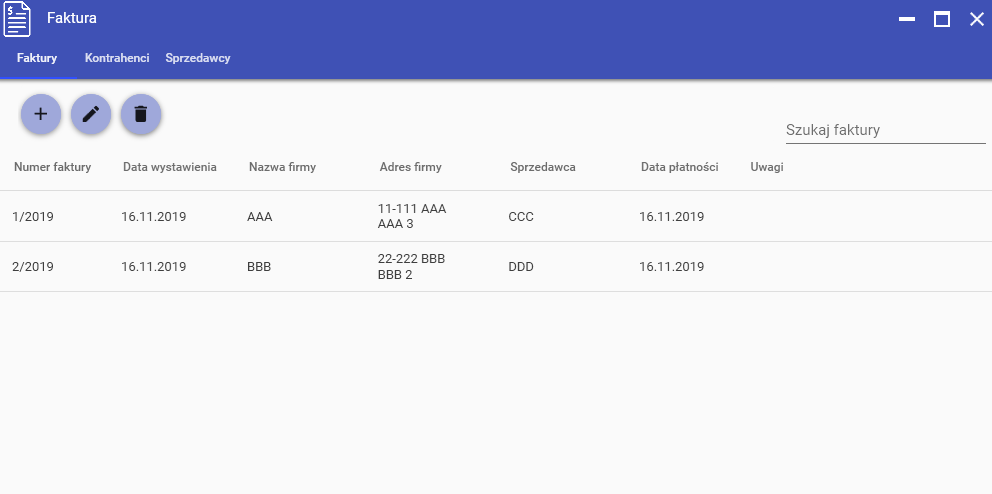
\includegraphics[width=\linewidth]{Rysunki/Main/InvoiceView.png}
  \caption{Okno widoku faktur}
  \label{fig:AddCustomerWindowInvoice}
\end{figure}

Aplikacja wyświetla nam wszystkie dostępne faktury \ref{fig:AddCustomerWindowInvoice}. Możemy zmienić widok na listę kontrahentów \ref{fig:AddCustomerWindowContractor} lub sprzedawców \ref{fig:AddCustomerWindowSeller}. 

\begin{figure}[ht!]
\centering
  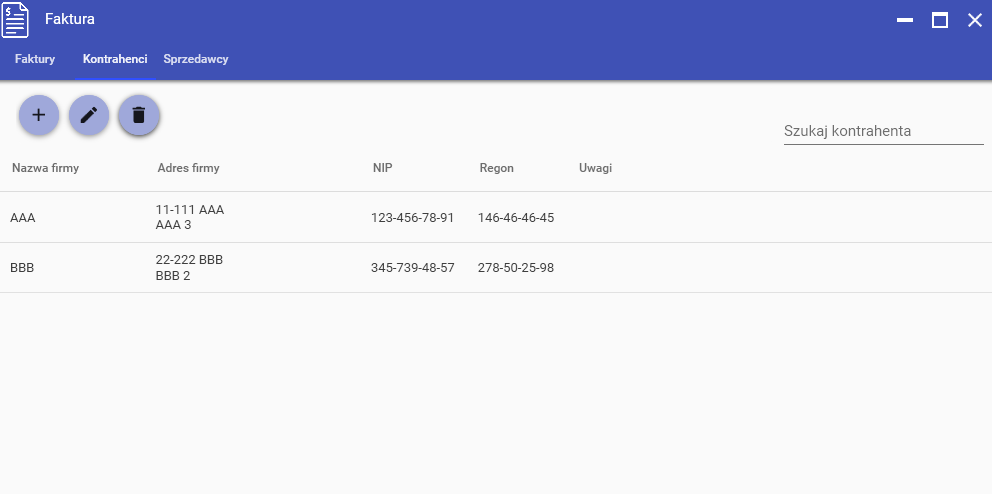
\includegraphics[width=\linewidth]{Rysunki/Main/contractorView.png}
  \caption{Okno widoku kontrahentów}
  \label{fig:AddCustomerWindowContractor}
\end{figure}

\begin{figure}[ht!]
\centering
  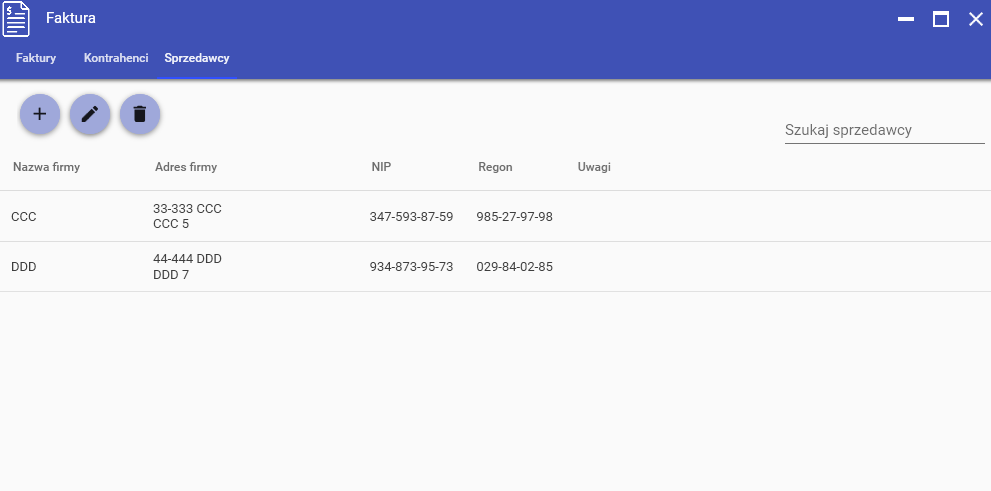
\includegraphics[width=\linewidth]{Rysunki/Main/sellerView.png}
  \caption{Okno widoku sprzedawców}
  \label{fig:AddCustomerWindowSeller}
\end{figure}

W każdym z tych trzech widoków możemy wykonać 3 takie same operacje - Dodanie, Edycja, Usunięcie. Każda z zakładek posiada również funkcjonalność szukania \ref{fig:AddCustomerWindowSearch}, która jest bardzo przydatna w przypadku dużej ilości pozycji na listach. Podczas usuwania faktury \ref{fig:AddCustomerWindowDeleteInvoice} użytkownikowi wyświetlany jest stosowny komunikat, który żąda potwierdzenia usunięcia faktury.

\begin{figure}[ht!]
\centering
  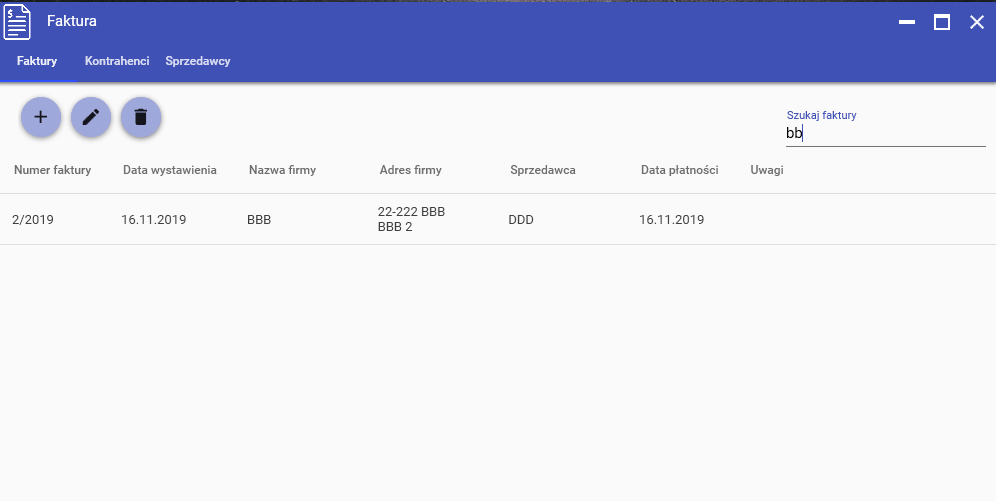
\includegraphics[width=\linewidth]{Rysunki/Main/MainSearch.png}
  \caption{Funkcja szukania}
  \label{fig:AddCustomerWindowSearch}
\end{figure}

\begin{figure}[ht!]
\centering
  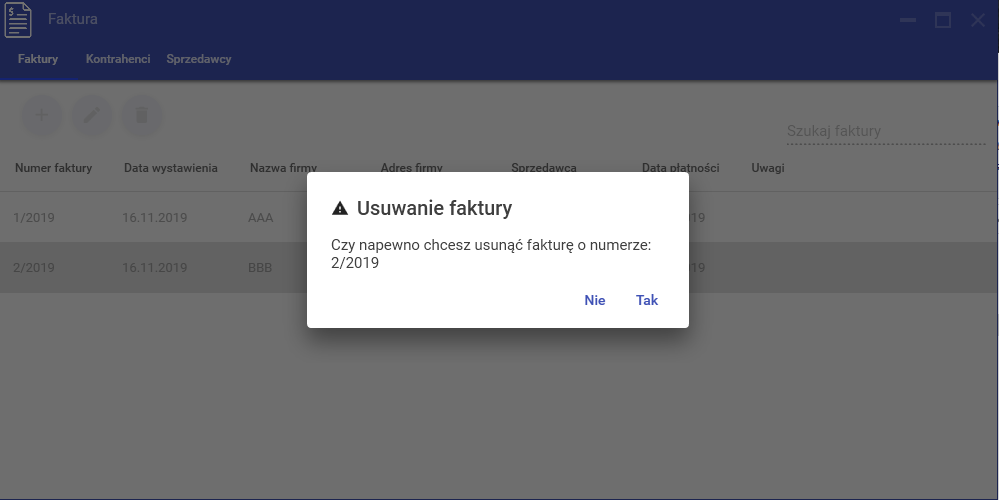
\includegraphics[width=\linewidth]{Rysunki/Main/deleteInvoiceView.png}
  \caption{Usuwanie faktury}
  \label{fig:AddCustomerWindowDeleteInvoice}
\end{figure}

\newpage~\newpage~\newpage~
\section{AddCustomerWindow}
Widok AddCustomerWindow jest oknem dodawania nowego kontrahenta lub sprzedawcy \ref{fig:AddCustomerWindow} (w zależności od tego jaki typ wybierzemy). 

\begin{figure}[ht!]
\centering
  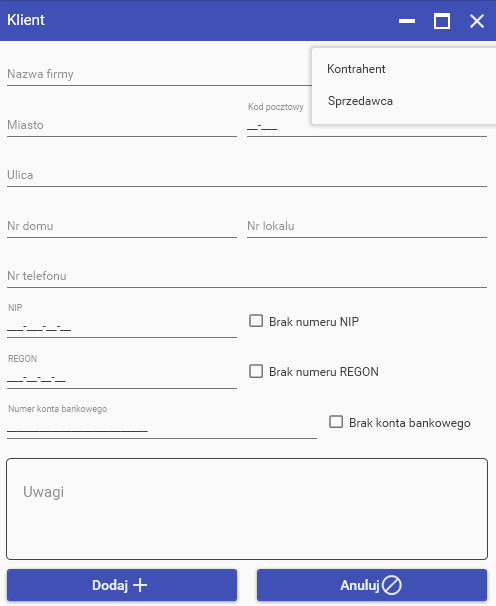
\includegraphics[width=0.7\linewidth]{Rysunki/AddCustomer/CustomerWindow.png}
  \caption{Okno widoku AddCustomerWindow}
  \label{fig:AddCustomerWindow}
\end{figure}

Wymaganymi wartościami do uzupełnienia są:

\begin{itemize}
    \item Nazwa firmy
    \item Miasto
    \item Ulica
    \item Numer domu
\end{itemize}

W przypadku, gdy nie podamy powyższych wartości nie będziemy w stanie zapisać nowego obiektu. Aplikacja wyświetli stosowny komunikat oraz zaznaczy pola, które zostały źle uzupełnione lub pominięte \ref{fig:AddCustomerWindowError}. 

\begin{figure}[ht!]
\centering
  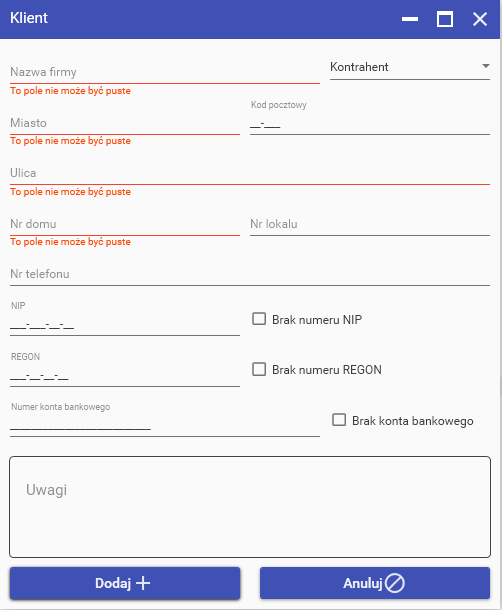
\includegraphics[width=0.7\linewidth]{Rysunki/AddCustomer/AddCustomerError.png}
  \caption{Widok pominiętych danych, które są wymagane}
  \label{fig:AddCustomerWindowError}
\end{figure}

\newpage~\newpage~
\section{InvoiceWindow}
Widok InvoiceWindow jest jednym z ważniejszych widoków w aplikacji. Na poniższym rysunku \ref{fig:InvoiceWindow} widoku możemy wybrać kontrahenta oraz sprzedawcę, na których będzie wypisana faktura. Następnie mamy możliwość wyboru daty wystawienia \ref{fig:InvoiceWindowDate} oraz zaznaczenia czy faktura będzie fakturą pro forma czy VAT. Poniżej wybieramy rodzaj płatności (gotówka, przelew lub płatność kartą), termin do kiedy faktura musi zostać opłacona oraz opcjonalnie (jeżeli została już opłacona) datę opłacenia faktury.

\begin{figure}[ht!]
\centering
  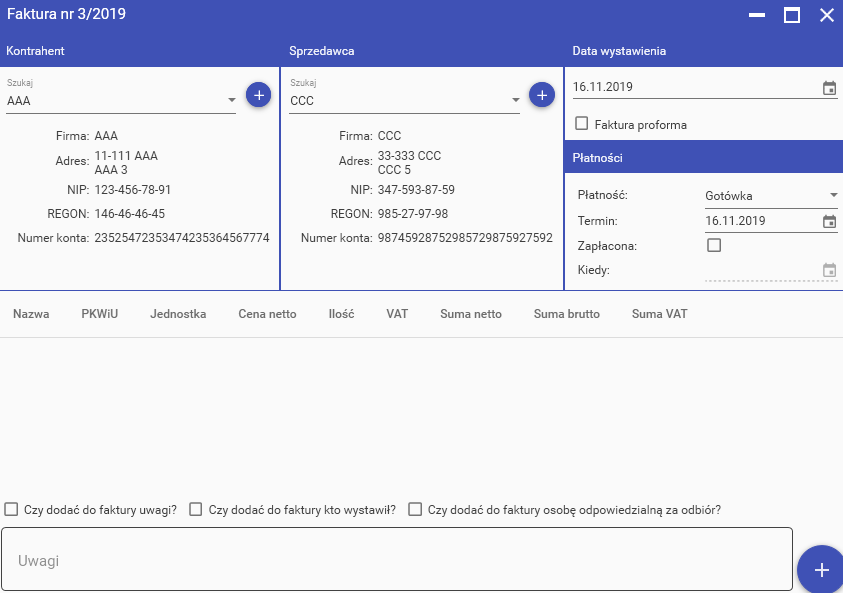
\includegraphics[width=\linewidth]{Rysunki/Invoice/InvoiceWindow.png}
  \caption{Okno widoku dodawania faktury}
  \label{fig:InvoiceWindow}
\end{figure}

\begin{figure}[ht!]
\centering
  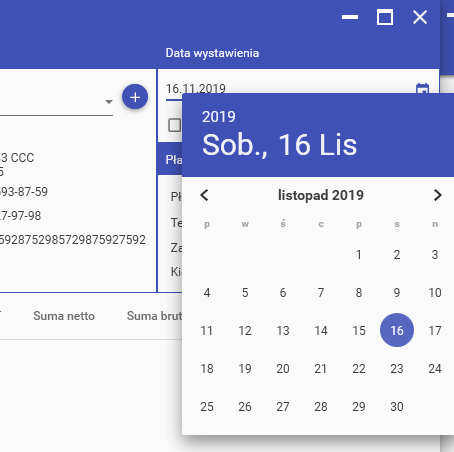
\includegraphics[width=0.5\linewidth]{Rysunki/Invoice/InvoiceSelectDate.png}
  \caption{Okno wyboru daty}
  \label{fig:InvoiceWindowDate}
\end{figure}

W prawym dolnym rogu znajduje się przycisk z ,,plusikiem'', który po kliknięciu otwiera nam menu opcji \ref{fig:InvoiceWindowMenu}. Pierwsze trzy przyciski służą do operacji na pozycjach znajdujących się na fakturze. Kolejne dwa pozwalają wygenerować fakturę VAT oraz jej korektę w przypadku jakichkolwiek zmian.

\begin{figure}[ht!]
\centering
  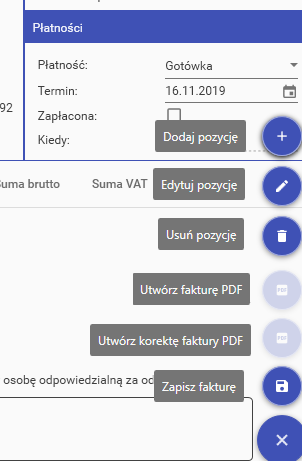
\includegraphics[width=0.5\linewidth]{Rysunki/Invoice/InvoiceMenu.png}
  \caption{Menu opcji na widoku InvoiceWindow}
  \label{fig:InvoiceWindowMenu}
\end{figure}

Rysunek \ref{fig:InvoiceWindowEdit} prezentuje nam fakturę w trybie podglądu. Na początku wszystkie kontrolki są wyłączone. W celu przejścia do trybu edycji użytkownik musi kliknąć przycisk ,,Edytuj fakturę''. W trybie podglądu aktywne są tylko 4 przyciski, które pozwalają na dodanie pól do pliku PDF z fakturą: 

\begin{itemize}
    \item Faktura proforma
    \item Czy dodać do faktury uwagi?
    \item Czy dodać do faktury kto wystawił?
    \item Czy dodać do faktury osobę odpowiedzialną za odbiór?
\end{itemize}

\begin{figure}[ht!]
\centering
  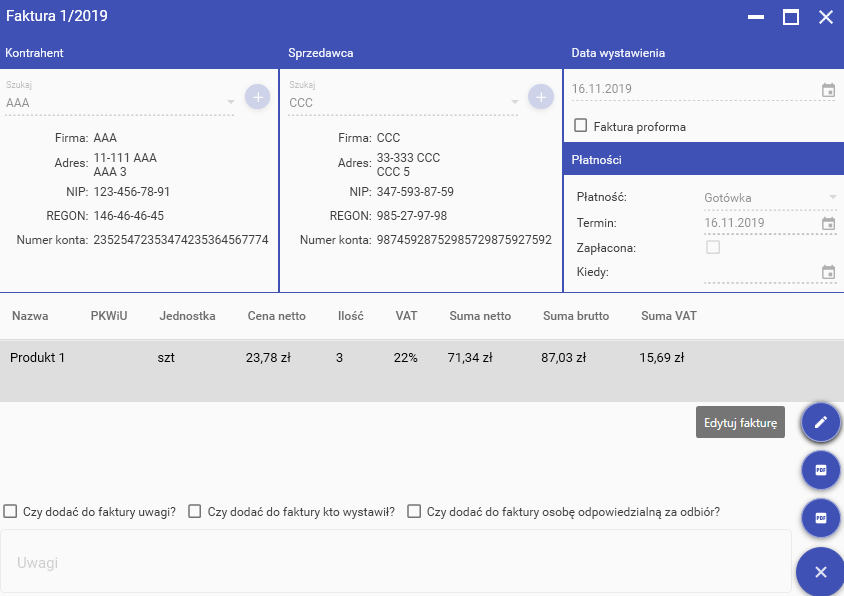
\includegraphics[width=\linewidth]{Rysunki/Invoice/InvoiceEdit.png}
  \caption{Okno widoku podglądu faktury}
  \label{fig:InvoiceWindowEdit}
\end{figure}

\newpage~\newpage~\newpage~
\section{InvoiceItemWindow}
Widok InvoiceItemWindow \ref{fig:InvoiceItemWindow} jest oknem dodawania pozycji do faktury.

\begin{figure}[ht!]
\centering
  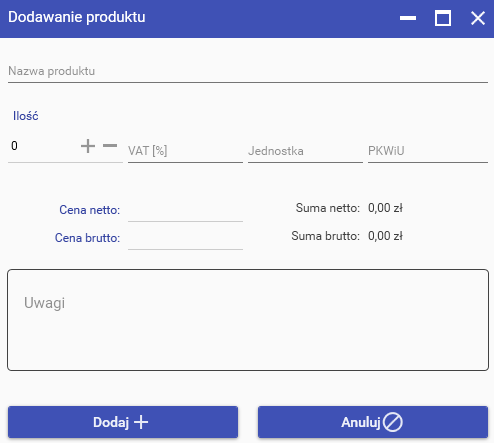
\includegraphics[width=\linewidth]{Rysunki/InvoiceItem/InvoiceItemWindow.png}
  \caption{Okno widoku dodawania pozycji do faktury}
  \label{fig:InvoiceItemWindow}
\end{figure}

Wymagane pola na widoku to InvoiceItemWindow to: 
\begin{itemize}
    \item Nazwa produktu
    \item VAT [\%]
    \item Jednostka
    \item Cenna netto lub brutto (jedna liczona na podstawie drugiej)
\end{itemize}

\newpage
W przypadku niepodania któregoś w powyższych pól, użytkownik otrzyma odpowiedni komunikat \ref{fig:InvoiceItemWindowError}.

\begin{figure}[ht!]
\centering
  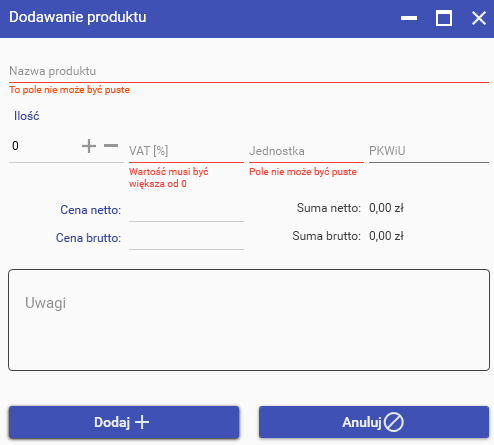
\includegraphics[width=\linewidth]{Rysunki/InvoiceItem/InvoiceItemWindowError.png}
  \caption{Błąd przy dodawaniu pozycji (niewypełnione pola)}
  \label{fig:InvoiceItemWindowError}
\end{figure}
\chapter{Podsumowanie}
Podstawowym celem pracy było napisanie aplikacji desktopowej pozwalającej na zarządzanie fakturami oraz danymi kontrahentów. Cel został w całości zrealizowany. Aplikacja pozwala na dodawanie, usuwanie oraz edycję faktur. Podobnie jest z danymi kontrahentów. Program pozwala również na wyszukiwanie oraz sortowanie faktur jak i kontrahentów. Wymagania funkcjonalne oraz niefunkcjonalne, które zostały postawione przed rozpoczęciem projektu, zostały zrealizowane. W aplikacji udało się zaimplementować najważniejszą funkcjonalność - generowanie plików PDF z faktur.

%\bibliographystyle{plalpha}
\bibliographystyle{plabbrv}

%UWAGA: bibliotekę referencji należy przygotować samemu. Dobrym do tego narzędziem jest JabRef.
%       Nazwę przygotowanej biblioteki wpisuje się poniżej bez rozszerzenia 
%       (w tym przypadku jest to "dokumentacja.bib")
\bibliography{dokumentacja}
\appendix
\chapter{Opis załączonej płyty CD/DVD}
Na płycie znajduje się kod źródłowy całej aplikacji, skompilowana wersja gotowa do uruchomienia na każdym komputerze oraz plik PDF z całą pracą inżynierską.

\chapterstyle{noNumbered}
\phantomsection % sets an anchor
\addcontentsline{toc}{chapter}{Indeks rzeczowy}
\printindex

\end{document}
